%
% 3-risch.tex
%
% (c) 2026 Prof Dr Andreas Müller
%
\section{Der Risch-Algorithmus
\label{buch:intalg:section:risch}}
\kopfrechts{Der Risch-Algorithmus}%
Das Liouville-Prinzip erklärt, wie ein Funktion aussehen muss, wenn sie
eine elementare Stammfunktion haben soll.
Für sich allein genommen reicht es nicht, für eine beliebige elementare
Funktion zu entscheiden, ob sie auch ein elementare Stammfunktion hat.
Dazu sind weitere Überlegungen nötig, die in diesem Kapitel dargestellt
werden sollen.
Das Ziel ist ein Entscheidungsalgorithmus, der ausgehend von einer
elementaren Funktion als Integranden schrittweise eine Stammfunktion
konstruiert.
Falls ein Schritt sich als nicht durchführbar erweist, bedeutet dies,
dass keine elementare Stammfunktion existiert.

Der Risch-Algorithmus entstand aus den Ansätzen, die Richard Henry Risch
in den Sechzigerjahren entwickelte \cite{buch:risch}.
Er beginnt mit einer Verallgemeinerung der Methode von Hermite zur
Behandlung des rationalen Teils.
Die besonders erfolgreiche Methode von Rothstein-Trager zur Bestimmung
der Koeffizienten $c_i$ und der Funktionen $v_i$ kam in den Siebzigerjahren
dazu.
Die folgende Darstellung des Algorithmus stützt sich weitgehend auf 
\cite{buch:algorithms}.

%
% Übersicht über den Algorithmus
%
\subsection{Übersicht über den Algorithmus
\label{buch:intalg:risch:uebersicht}}
Bevor wir die notwendigerweise unterschiedlichen Vorgehensweisen 
für logarithmische, exponentielle und algebraische Erweiterungen
im Detail betrachten, wollen wir in diesem Abschnitt die für alle
Fälle gemeinsame prinzipielle Vorgehensweise
des Algorithmus skizzieren.

%
% Die Aufgabenstellung
%
\subsubsection{Die Aufgabenstellung}
Es ist ein Algorithmus zu entwickeln, der zu einer elementaren Funktion
eine elementare Stammfunktion findet, sofern eine solche existiert.
Falls keine elementare Stammfunktion existiert, soll der Algorithmus
einen Beweis für diese Tatsache konstruieren.
Um dieses Ziel zu erreichen, muss zunächst klargestellt werden, welche
Funktionen als Integranden in Frage kommen sollen.

Zu den Funktionen, die als Stammfunktionen zugelassen werden sollen,
sollen mindestens alle rationalen Funktionen mit rationalen Koeffizienten
gehören.
Wir gehen also von einem Funktionenkörper aus, der eine Erweiterung
von $\mathbb{Q}$ um ein transzendentes Element $x$ ist, welches die
Eigenschaft $Dx=1$ hat.
Dieser Körper wird auch mit $\mathbb{Q}(x)$ bezeichnet.

Ein typisches Computeralgebrasystem wird noch weitere Konstanten
als Koeffizienten der rationalen Funktionen zulassen, zum Beispiel
Naturkonstanten wie $g$ oder $c$, denen man zwar auch einen numerischen
Wert zuordnen kann, aber man interessiert sich durchaus auch dafür, 
wie solche Konstanten in die Stammfunktion eingehen können.
Solche Konstanten können als transzendente Erweiterungen des Körpers
$\mathbb{Q}$ angesehen werden, die zusätzlich die Eigenschaft haben,
dass ihre Ableitung verschwindet.
Weiter ist es möglich, dass zusätzliche mathematische Konstanten
benötigt werden.
Diese können sowohl transzendente Erweiterungen sein wie $\pi$, $e$,
$\zeta(2)=\pi^2/6$ oder $\zeta(3)$, oder sie können algebraisch sein wie
$\!\sqrt{2}$ oder $\sqrt[3]{7}$.
Die algebraische Abhängigkeit dieser Konstanten untereinander wird
nicht weiter untersucht und hat auch keinen Einfluss auf das
Integrationsproblem.

Innerhalb des Konstantenkörpers kann es durchaus passieren, dass eine
transzendente Konstante in einer algebraischen Erweiterung von
$\mathbb{Q}$ liegt.
Dies passiert zum Beispiel für die transzendente Konstate $\pi$,
$\mathbb{Q}\subset \mathbb{Q}(\pi)$ ist eine transzendente Erweiterung.
Sie enthält auch $\zeta(2) = \pi^2/6$.
Andererseits ist $\mathbb{Q}(\zeta(2)) \subset \mathbb{Q}(\zeta(2),\pi)$
eine algebraische Erweiterung, da $\pi$ eine Nullstelle des Polynoms
\[
p(X)
=
X^2 - 6\zeta(2)
=
X^2 - \pi^2
\qquad
\Rightarrow
\qquad
p(\pi)=0
\]
ist.
Während $\mathbb{Q}(\pi)$ auch $\zeta(2)$ bereits enthält, braucht
es eine algebraische Erweiterung von $\mathbb{Q}(\zeta(2))$, um $\pi$
zu finden.
Im Folgenden nehmen wir an, dass alle nötigen Konstanten von Anfang
an dem Körper $\mathbb{Q}$ hinzugefügt worden sind und den Konstantenkörper
$K$ bilden.

Es ist auch denkbar, dass während der Bestimmung der Stammfunktion weitere
Konstanten benötig werden. 
Zum Beispiel kann es nötig sein, ein Polynom zu faktorisieren.
Die dabei gefundenen Nullstellen sind algebraische Konstanten über
dem Körper $K$.
Dazu gehört insbesondere auch das Element $i$ mit $i^2=-1$, welches
zum Beispiel für die Konstruktion der trigonometrischen Funktionen
benötigt wird.
Auch diese Konstanten sollen von Anfang an in $K$ enthalten sein, so
dass es später nicht mehr nötig ist, den Konstantenkörper zu erweitern.

Die Konstruktion des differentiellen Funktionenkörpers beginnt daher
mit dem trans\-zen\-den\-ten Element $x$ und dem Körper $F=K(x)$ der rationalen
Funktionen in $x$ mit Koeffizienten in $K$.
Diesem Körper werden jetzt weiter drei Arten von Funktionen hinzugefügt:
\begin{itemize}
\item
Logarithmische transzendente Erweiterungen: Dies sind Funktionen $\vartheta=\log u$,
die durch die Eigenschaft $D\vartheta= Du/u$ bis auf eine Konstante
definiert sind.
\item
Exponentielle transzendente Erweiterungen: Dies sind Funktionen $\vartheta=e^u$,
die durch die Eigenschaft $D\vartheta = \vartheta\cdot Du$ bis auf einen
skalaren Faktor definiert sind.
\item
Algebraische Elemente: Dies sind Funktionen $\vartheta$, die eine algebraische
Gleichung
\[
a_n\vartheta^n + a_{n-1}\vartheta^{n-1} + \dots + a_1\vartheta + a_0 = 0
\]
erfüllen.
\end{itemize}
Um einen zulässigen Integranden oder eine Stammfunktion zu konstruieren,
kann es notwendig sein, mehrere solche Erweiterungen hinzufügen, die auch
von verschiedener Art sein können.
Wir haben also mit einer Folge von Erweiterungen
\[
F
\subset
\underbrace{
F(\vartheta_1)
}_{\displaystyle = F_1}
\subset
\underbrace{
F(\vartheta_1,\vartheta_2)
}_{\displaystyle = F_2}
\subset
\dots
\subset
\underbrace{
F(\vartheta_1,\vartheta_2,\dots,\vartheta_n)
}_{\displaystyle=F_n}
\]
zu tun.
Insbesondere ist auch
\[
F_n = F_{n-1}(\vartheta_n)=F(\vartheta_1,\dots,\vartheta_{n-1})(\vartheta_n).
\]
Dieser Aufbau des Funktionenkörpers durch wiederholte Adjunktion von 
logarithmischen, exponentiellen oder algebraischen Elementen war auch
bereits der Rahmen, in dem das Liouville-Prinzip formuliert und im
Abschnitt~\ref{buch:intalg:liouville:subsection:allgemein}
bewiesen wurde.

Mit den Differentialkörpern $F_k$ kann jetzt die Aufgabenstellung 
genauer formuliert werden.
Zu einer Funktion $f\in F_n$ soll der Algorithmus eine Stammfunktion
$g\in F_n$ finden, also eine Funktion $Dg=f$.
Falls keine solche Funktion existiert, soll er einen Beweis dafür
konstruieren.

%
% Der polynomielle und der rationale Teil
%
\subsubsection{Der polynomielle und der rationale Teil}
Wir betrachten eine Funktion $f\in F_n = F_{n-1}(\vartheta_n)$ und
versuchen die Frage zu beantworten, ob $f$ eine Stammfunktion in
$F_n$ hat.
Dies bedeutet, dass $f$ als eine rationale Funktion der Form
\begin{equation}
f
= 
\frac{p(\vartheta_n)}{q(\vartheta_n)},
\qquad
p(\vartheta_n), q(\vartheta_n)\in F_{n-1}[\vartheta_n]
\label{buch:intalg:risch:uebersicht:eqn:integrand}
\end{equation}
geschrieben werden kann.
Im Gegensatz zur Situation in Kapitel~\ref{chapter:ratint}, wo rationale
Funktionen mit konstanten Koeffizienten untersucht wurden, haben
die Polynome $p(\vartheta_n)$ und $q(\vartheta_n)$ Koeffizienten
in $F_{n-1}$, sind also selbst Funktionen.

Auf die Polynome im Integranden
\eqref{buch:intalg:risch:uebersicht:eqn:integrand}
kann der Polynomdivisionsalgorithmus angewendet werden, was auf die
Zerlegung
\[
\frac{p(\vartheta_n)}{q(\vartheta_n)}
=
s(\vartheta_n)
+
\frac{r(\vartheta_n)}{q(\vartheta_n)},
\qquad
s(\vartheta_n), q(\vartheta_n) \in F_{n-1}[\vartheta_n],
\]
führt.
Das Polynom $r(\vartheta_n)$ hat Grad
$\deg r(\vartheta_n) < \deg q(\vartheta_n)$.
Wir nennen $s(\vartheta_n)$ den polynomiellen Teil und den Bruch
den rationalen Teil.

Das gesuchte Integral kann jetzt in die zwei Integrale
\[
\int f
=
\int
\frac{p(\vartheta_n)}{q(\vartheta_n)}
=
\underbrace{
\int s(\vartheta_n)
}_{\displaystyle\text{polynomieller Teil\strut}}
+
\underbrace{
\int
\smash{\frac{r(\vartheta_n)}{q(\vartheta_n)}}.
}_{\displaystyle\text{rationaler Teil\strut}}
\]
zerlegt werden.
Im Falle rationaler Funktionen war der polynomielle Teil sehr einfach
auszuführen, da $\int z^n=z^{n+1}/(n+1)$.
Im vorliegenden, allgemeineren Fall wird eine neue Methode nötig.
Schon das einfache Polynom $s(\vartheta_n) = \vartheta_n$ führt auf
das nichttriviale Integral $\int s(\vartheta_n) = \int\vartheta_n$.
Wegen der sehr unterschiedlichen Eigenschaften der verschiedenen Arten
von Erweiterungen wird dies jeweils unterschiedliche Vorgehensweisen
erfordern, die in den nachfolgenen Abschnitten für jede Erweiterung
separat entwickelt werden müssen.
Die in Kapitel~\ref{chapter:ratint} mit einer Randbemerkung erledigte
Behandlung des polynomiellen Teils muss daher nochmals neu aufgerollt
werden und wird zu zusätzlichen Einschränkungen für die Existenz
einer Stammfunktion führen.

Für den rationalen Teil können wir ebenfalls versuchen, die
bereits bekannten Techniken anzuwenden.
Wir können eine quadratfreie Faktorisierung des Nenners $q(\vartheta_n)$
in Faktoren $b_k(\vartheta_n)\in F_{n-1}[\vartheta_n]$ vornehmen und
damit den Bruch in Partialbrüche aufteilen.
Weiter können wir die Methode von Hermite auf die Partialbrüche 
anwenden und damit den Nennerexponenten auf $1$ reduzieren.
Schliesslich können wir die Methode von Rothstein-Trager anwenden,
um die Koeffizienten $c_i$ und die Funktion $v_i\in F_{n-1}$ für
die Liouville-Darstellung der Stammfunktion zu finden.
Dabei wird sich allerdings eine neue Einschränkung ergeben, die darauf
beruht, dass die $c_i$, die die Methode von Rothstein-Trager findet,
Konstanten sein müssen.
Da die Koeffizienten der Zähler- und Nennerpolynome nicht konstant sein
müssen, könnten sich auch nicht konstante $c_i$ ergeben, was dann
beweist, dass die Stammfunktion nicht existieren kann.

Der Integrationsalgorithmus in $F_n$ folgt also ziemlich genau der
Vorgehensweise des Integrationsalgorithmus in $K(z)$.
Um die Notation zu vereinfachen, ist es daher angebracht, $F=F_{n-1}$
und $\vartheta=\vartheta_{n}$ zu setzen.
Zu $f\in F(\vartheta)=F_{n-1}(\vartheta_n)=F_n$ ist dann eine Stammfunktion
in $F(\vartheta)$ gesucht.
Im Gegensatz zur Situation in Kapitel~\ref{chapter:ratint} ist
aber nicht garantiert, dass die Stammfunktion tatsächlich existiert.

%
% Die Methode von Hermite
%
\subsubsection{Die Methode von Hermite}
Die Methode von Hermite verwendet eine quadratfreie Faktorisierung 
\[
q(\vartheta)
=
b_1(\vartheta) b_2(\vartheta)^2 \cdots b_m(\vartheta)^m,
\]
in der jeder Faktor $b_k(\vartheta)$ quadratfrei ist.
Zu dieser Faktorisierung gibt es immer eine Partialbruchzerlegung
\begin{equation}
\frac{r(\vartheta)}{q(\vartheta)}
=
\sum_{i=1}^m \sum_{k=1}^i \frac{a_{ik}(\vartheta)}{b_i(\vartheta)^k}
\end{equation}
mit $a_{ik}(\vartheta)\in F[\vartheta]$ und
$\deg a_{ik}(\vartheta)<\deg b_i(\vartheta)$.
Das Integral des rationalen Teils ist damit
\begin{equation}
\int
\frac{r(\vartheta)}{q(\vartheta)}
=
\sum_{i=1}^m \sum_{k=1}^i
\int \frac{a_{ik}(\vartheta)}{b_i(\vartheta)^k}.
\end{equation}
Es ist also nötig, Integrale der Form
\begin{equation}
\int \frac{a(\vartheta)}{b(\vartheta)^k}
\qquad
\text{mit $
a(\vartheta), b(\vartheta)\in F[\vartheta]
$}
\label{buch:intalg:risch:eqn:ratpart}
\end{equation}
zu bestimmen, mit dem quadratfreien Nennerpolynom
$b(\vartheta)$ mit $\deg a(\vartheta) < \deg b(\vartheta)$.
Die Methode von Hermite versucht, die
Integrale~\eqref{buch:intalg:risch:eqn:ratpart}
zu vereinfachen, indem der Nennerexponent $k$ reduziert wird.

Da $b(\vartheta)$ quadratfrei ist, sind $b(\vartheta)$ und $Db(\vartheta)$
in den meisten Fällen teilerfremd.
Die Fälle von Faktoren $\vartheta$ des Nennerpolynoms, in denen dies nicht
zutrifft, hängen von der Art der Erweiterung $\vartheta$ ab und werden
später separat diskutiert.
Teilerfremdheit hat zur Folge, dass es Polynome $s(\vartheta)$ und
$t(\vartheta)$ gibt mit
\[
a(\vartheta)
=
s(\vartheta) b(\vartheta)
+
t(\vartheta) Db(\vartheta).
\]
Damit wird das Integral zu
\begin{align*}
\int
\frac{a(\vartheta)}{b(\vartheta)^k}
&=
\int
\frac{s(\vartheta)}{b(\vartheta)^{k-1}}
+
\int t(\vartheta)\frac{Db(\vartheta)}{b(\vartheta)^k}
\intertext{und mit partieller Integration wird daraus}
&=
\int
\frac{s(\vartheta)-Dt(\vartheta)/(k-1)}{b(\vartheta)^{k-1}}
+
\frac{t(\vartheta)/(k-1)}{b(\vartheta)^{k-1}}.
\end{align*}
Der Zähler des ersten Integrals hat möglicherweise grösseren Grad
als $b(\vartheta)$.
Die Polynomdivision macht daraus einen zusätzlichen Beitrag zum polynomiellen
Teil.
Es bleibt das Problem, Integrale der Form~\eqref{buch:intalg:risch:eqn:ratpart}
mit $k-1$ anstelle von $k$ zu bestimmen.

Durch wiederholte Anwendung dieser Methode ist das Problem damit reduziert
auf Integrale der Form
\[
\int\frac{a(\vartheta)}{b(\vartheta)},
\qquad
a(\vartheta), b(\vartheta) \in F[\vartheta],
\]
wobei $b(\vartheta)$ quadratfrei ist.

%
% b(\vartheta) und Db(\vartheta)
%
\subsubsection{$b(\vartheta)$ und $Db(\vartheta)$}
Der entscheidende Schritt für die Durchführbarkeit der Methode von Hermite 
war die Garantie, dass
\[
a(\vartheta)
=
s(\vartheta) b(\vartheta)
+
t(\vartheta) Db(\vartheta)
\]
geschrieben werden kann.
Falls $b(\vartheta)$ und $Db(\vartheta)$ teilerfremd sind, dann gilt
dies nach dem erweiterten euklidischen Algorithmus tatsächlich.
Für ein quadratfreies Polynom in $u(X)\in K[X]$ wissen wir auch bereits,
dass $u(X)$ und das abgeleitete Polynom $u'(X)$
(siehe Definition~\ref{buch:intalg:elementar:def:abgeleitetespolynom})
teilerfremd sind.
Bei der Ableitung $Db(\vartheta)$ werden aber nicht nur die Potenzen
$\vartheta^k$ abgeleitet, sondern auch die Koeffizienten des Polynoms.

Man beachte, dass $Db(\vartheta)$ und $b'(\vartheta)$ verschieden sind.
Nach Definition~\ref{buch:intalg:elementar:def:abgeleitetespolynom} gilt
\begin{align*}
Db(\vartheta)
&=
\sum_{k=0}^m
D(b_k\vartheta^k)
\\
&=
\sum_{k=0}^m
\Bigl(
Db_k\vartheta^k
+
b_kk D\vartheta\cdot \vartheta^{k-1}
\Bigr)
\\
&=
\sum_{k=1}^m (Db_k)\vartheta^k
+
b'(\vartheta) D\vartheta.
\end{align*}
Da $D\vartheta$ auf der rechten Seite vorkommt, ist zunächst nicht einmal
klar, dass die rechte Seite auch wieder ein Polynom in $\vartheta$ mit
Koeffizienten in $F$ ist.
Dies muss später für jede Art von Erweiterung einzeln nachgeprüft werden.

Aus der Quadratfreiheit von $b(\vartheta)$ als Polynom in $F[\vartheta]$
folgt nur, dass $b(\vartheta)$ und $b'(\vartheta)$ teilerfremd sind.
Damit die Methode von Hermite durchführbar wird, muss also untersucht
werden, ob aus der Teilerfreiheit von $b(\vartheta)$ und $b'(\vartheta)$
auch folgt, dass $b(\vartheta)$ und $Db(\vartheta)$ teilerfremd sind.
Dies wird für logarithmische Erweiterungen in
Lemma~\ref{buch:intalg:risch:log:lemma:bDb} und für exponentielle
Erweiterungen in
Lemma~\ref{buch:intalg:risch:exp:lemma:bDb} durchgeführt.

%
% Standardform der Stammfunktion
%
\subsubsection{Standardform der Stammfunktion}
Die Methode von Rothstein-Trager von
Satz~\ref{buch:ratint:rothsteintrager:satz:rothsteintrager}
bestimmt die Stammfunktion einer rationalen Funktion mit quadratfreiem
Nenner und einem Zähler kleineren Grades und integriert damit den
rationalen Teil eines rationalen Integranden.
Die Methode soll auf Funktionen 
\begin{equation}
\frac{a(\vartheta)}{b(\vartheta)}
\qquad \text{mit}\quad \left\{
\begin{array}{l}
a(\vartheta),b(\vartheta)\in F[\vartheta],\\
\text{$a(\vartheta)$ und $b(\vartheta)$ teilerfremd,}\\
\text{$b(\vartheta)$ quadratfrei und normiert,}\\
\deg a(\vartheta) < \deg b(\vartheta)\\
\end{array}
\right.
\label{buch:intalg:risch:eqn:a(theta)/b(theta)}
\end{equation}
ausgedehnt werden.
Möglicherweise müssen die zulässigen Nenner $b(\vartheta)$ weiter
eingeschränkt werden.
Zum Beispiel wird sich herausstellen, dass bei einer exponentiellen
Erweiterung $\vartheta$ für den rationalen Teil eines
Integrals nur Nenner $b(\vartheta)$ zulässig sind, die nicht durch
$\vartheta$ teilbar sind.
Wir sagen, dass \eqref{buch:intalg:risch:eqn:a(theta)/b(theta)}
ein \emph{rationaler Teil} für die Körpererweiterung $F\subset F(\vartheta)$
ist, wenn $b(\vartheta)$ ein zulässiger Nenner ist.

Nach dem Liouville-Prinzip muss die Stammfunktion, falls sie elementar ist,
die Form
\begin{equation}
\int
\frac{a(\vartheta)}{b(\vartheta)}
=
v_0(\vartheta)
+
\sum_k c_k\log v_k(\vartheta)
\label{buch:intalg:risch:rt:eqn:liouvilleint}
\end{equation}
haben.
Für den Integranden muss entsprechend gelten, dass
\begin{equation}
\frac{a(\vartheta)}{b(\vartheta)}
=
Dv_0(\vartheta)
+
\sum_k c_k\frac{D v_k(\vartheta)}{v_k(\vartheta)}
\label{buch:intalg:risch:rt:eqn:liouvillediff}
\end{equation}
ist.
Darin sind die $c_k$ Konstanten und $v_k(\vartheta)\in F(\vartheta)$.
Die Methode von Rothstein-Trager findet die $c_k$ und die $v_k(\vartheta)$.

Die Darstellung
\eqref{buch:intalg:risch:rt:eqn:liouvilleint}
der Stammfunktion ist nicht die einzig mögliche.
Auch bei der Integration rationaler Funktionen waren Umformungen
verwendet worden, um der Stammfunktion genau die Form zu geben,
die die Methode von Rothstein-Trager später fand.
Im Folgenden sollen ähnliche Vereinheitlichungen für die Darstellung
\eqref{buch:intalg:risch:rt:eqn:liouvilleint}
vorgenommen werden.

In der Darstellung \eqref{buch:intalg:risch:rt:eqn:liouvilleint}
der Stammfunktion sind die $v_k(\vartheta) \in F(\vartheta)$ rationale
Funktionen von $\vartheta$.
Im Beweis des
Satzes~\ref{buch:ratint:rothsteintrager:satz:rothsteintrager}
über die Stammfunktion rationaler Funktionen
wurde das Wissen aus der Methode von Bernoulli verwendet, dass die
\index{Bernoulli, Methode von}%
\index{Methode von Bernoulli}%
\index{Bernoulli, Johann}%
$v_k$ auch als normierte Polynome gewählt werden können.
Dies trifft aber auch im vorliegenden Fall zu.
Sind nämlich die $v_k(\vartheta)$ Brüche
\[
v_k(\vartheta)
=
\frac{z_k(\vartheta)}{w_k(\vartheta)}
\]
von Zähler $z_k(\vartheta)$ und Nenner $w_k(\vartheta)$
mit $z_k(\vartheta), w_k(\vartheta)\in F[\vartheta]$, dann können
wir \eqref{buch:intalg:risch:rt:eqn:liouvilleint} in der Form
\begin{equation*}
\int
\frac{a(\vartheta)}{b(\vartheta)}
=
v_0(\vartheta)
+
\sum_k c_k\log v_k(\vartheta)
=
v_0(\vartheta)
+
\sum_k c_k\log z_k(\vartheta)
-
\sum_k c_k\log w_k(\vartheta)
\end{equation*}
schreiben.
Die Argumente der Logarithmen sind jetzt sogar Polynome $\vartheta$.
Dies zeigt, dass man annehmen darf, dass in
\eqref{buch:intalg:risch:rt:eqn:liouvilleint}
$v_k(\vartheta)\in F[\vartheta]$ gilt.

Wir möchten zeigen, dass man annehmen darf, dass $v_k(\vartheta)$
normiert ist.
Dazu schreiben wir
$v_k(\vartheta) = v_{\deg v_0(\vartheta)} \bar{v}_k(\vartheta)$, worin
$\bar{v}_k(\vartheta)$ ein normiertes Polynom ist.
Dann ist
\[
c_k\log v_k(\vartheta)
=
c_k\log v_{\deg v_k(\vartheta)}
+
c_k\log \bar{v}_k(\vartheta).
\]
Indem wir den Ausdruck $c_k\log v_{\deg v_k(\vartheta)}\in F$ zu
$v_0(\vartheta)$ hinzufügen, können wir annehmen, das $v_k(\vartheta)$
\emph{normiert} ist.

Falls mehrere der Koeffizienten $c_k$ gleich sind, dann können wir 
die zugehörigen Funktionen $v_k$ zusammenfassen.
Zu gegebenem $c$ schreiben wir daher
\[
v(\vartheta) = \prod_{c_k=c} v_k(\vartheta).
\]
Dann ist
\begin{align*}
c \log v(\vartheta)
&=
c
\log\biggl(\prod_{c_k=c} v_k(\vartheta)\biggr)
=
\sum_{c_k=c} c_k \log v_k(\vartheta)
\intertext{mit der Ableitung}
c \frac{Dv(\vartheta)}{v(\vartheta)}
&=
D(c\log v(\vartheta))
=
\sum_{c_k=c} c_k \frac{Dv_k(\vartheta)}{v_k(\vartheta)}.
\end{align*}
Man darf also immer annehmen, dass die $c_k$ in der Liouville-Form der
Stammfunktion alle \emph{verschieden} sind.

Falls zwei Polynome $v_k(\vartheta)$ und $v_l(\vartheta)$ einen nichttrivialen
gemeinsamen Faktor haben, dann können wir mit
$g(\vartheta)=\operatorname{ggT}(v_k(\vartheta),v_l(\vartheta))$
\[
v_k(\vartheta) = w_k(\vartheta) g(\vartheta)
\qquad\text{und}\qquad
v_l(\vartheta) = w_l(\vartheta) g(\vartheta)
\]
schreiben.
Es gilt dann
\[
c_i\log v_i(\vartheta) + c_j\log v_j(\vartheta)
=
c_i\log w_i(\vartheta) + c_j \log w_j(\vartheta) + (c_i+c_j)\log g(\vartheta).
\]
Die Argumente der Logarithmen auf der rechten Seite haben keine 
gemeinsamen Faktoren.
Man darf also annehmen, dass die $v_k(\vartheta)$ \emph{teilerfremd} sind.

Falls $v_k(\vartheta)$ mehrfache Faktoren hat, können diese wie folgt
eliminiert werden.
In der quadratfreien Faktorisierung
\[
v_k(\vartheta) = p_0 p_1(\vartheta) p_2(\vartheta)^2 \dots p_l(\vartheta)^l
\]
von $v_k(\vartheta)$ sind alle Faktoren $p_i(\vartheta)\in F[\vartheta]$
quadratfrei.
Der Logarithmus ist
\[
\log v_k(\vartheta)
=
\log p_0
+
\log p_1(\vartheta)
+
2 \log p_2(\vartheta)
+
\dots
+
l\log p_l(\vartheta)
\]
ein Summe mit lauter quadratfreien Argumenten des Logarithmus.
Man darf also annehmen, dass die $v_k(\vartheta)$ sogar \emph{quadratfrei} sind.

Der Term $v_0(\vartheta)$ kam in der Methode von Rothstein-Trager für
rationale Funktionen nicht vor, da diese nur den logarithmischen Teil
geliefert hat.
Im vorliegenden Fall ist die Sachlage etwas komplizierter.
Sie wird geklärt durch die folgenden zwei Lemmata, sie später
in den Abschnitten~\ref{buch:intalg:risch:logarithmisch}
und \ref{buch:intalg:risch:exponentiell}
für logarithmische bzw.~exponentielle Erweiterungen bewiesen.

\begin{lemma}
\label{buch:intalg:risch:lemma:v0log}
Ist $\vartheta$ eine logarithmische Körpererweiterung von $F$, dann ist
in der Stammfunktion 
\eqref{buch:intalg:risch:rt:eqn:liouvilleint}
eines rationalen Teils immer $v_0(\vartheta)=0$.
\end{lemma}

\begin{lemma}
\label{buch:intalg:risch:lemma:v0exp}
Ist $\vartheta$ eine exponentielle Körpererweiterung von $F$ mit
$D\vartheta = \vartheta Du$, dann ist in der Stammfunktion 
\eqref{buch:intalg:risch:rt:eqn:liouvilleint}
eines rationalen Teils immer $v_0(\vartheta)\in F$.
\end{lemma}

Mit diesen zwei Lemmata ausgerüstet können wir jetzt wieder zeigen,
dass die $v_k(\vartheta)$ so gewählt werden können, dass $b(\vartheta)$
das Produkt der $v_k(\vartheta)$ ist.
Zu diesem Zweck nehmen wir an, dass
\begin{equation}
\frac{a(\vartheta)}{b(\vartheta)}
=
v_0 + \sum_{i=1}^m c_k \frac{Dv_k(\vartheta)}{v_k(\vartheta)},
\label{buch:intalg:risch:uebersicht:eqn:stammfunktion}
\end{equation}
und
verwenden wir die Notation
\[
u_k(\vartheta)
=
\prod_{\scriptstyle i=1\atop\scriptstyle i\ne k} v_i(\vartheta)
\qquad\text{und}\qquad
v(\vartheta)
=
\prod_{i=1} v_i(\vartheta).
\]
Wir wollen zeigen, dass $b(\vartheta)=v(\vartheta)$.

Wir multiplizieren \eqref{buch:intalg:risch:uebersicht:eqn:stammfunktion}
mit $b(\vartheta)$ und $v(\vartheta)$ und erhalten
\[
a(\vartheta) v(\vartheta)
=
v_0 b(\vartheta) \prod_{i=1}^m v_i(\vartheta)
+
\sum_{i=1}^m Dv_i(\vartheta) u_i(\vartheta) b(\vartheta).
\]
$b(\vartheta)$ teilt jeden Term auf der rechten Seite, ist aber teilerfremd
zu $a(\vartheta)$, also muss $b(\vartheta)\mid a(\vartheta)$ teilen.
Andererseits teilt $v_k(\vartheta)$ die linke Seite, den ersten Term
auf der rechten Seite und alle Terme der Summe ausser dem Term mit $i=k$.
Daher muss $v_k(\vartheta)$ auch letzteren Term
\[
c_k Dv_k(\vartheta) u_k(\vartheta) b(\vartheta)
\]
teilen.

Für logarithmische Erweiterungen folgt jetzt bereits aus der Quadratfreiheit
von $v_k(\vartheta)$, dass $v_k(\vartheta) \mid b(\vartheta)$.
Für exponentielle Erweiterungen könnte $v_k(\vartheta)$ auch ein
Teiler von $Dv_k(\vartheta)$ sein.
Dann müsste aber $v_k(\vartheta)$ ein Monom sein, was nicht zulässig
ist, weil der Faktor $\vartheta$ von $b(\vartheta)$ für exponentielle
Erweiterungen ausgeschlossen wurde.
Da jeder Faktor $v_k(\vartheta)$ ein Teiler ist, gilt auch
$v(\vartheta)\mid b(\vartheta)$.
Da sowohl $b(\vartheta)$ wie auch $v(\vartheta)$ normiert sind, folgt
$b(\vartheta) = v(\vartheta)$.

Wir fassen die gefundenen Standardisierungen der Stammfunktion im folgenden
Satz zusammen.

\begin{satz}[Standardform]
\label{buch:intalg:risch:satz:standardform}
\index{Satz!über die Standardform}%
Sei $\vartheta$ eine logarithmische oder exponentielle Erweiterung.
Falls der rationale Teil $a(\vartheta)/b(\vartheta)$ eine elementare
Stammfunktion hat, dann gibt es $v_0\in F$ und normierte, quadratfreie,
paarweise teilerfremde Polynome $v_k(\vartheta)\in F[\vartheta]$ mit
\begin{equation}
\frac{a(\vartheta)}{b(\vartheta)}
=
v_0 + \sum_{k=1}^m \frac{Dv_k(\vartheta)}{v_k(\vartheta)}
\qquad\text{und}\qquad
b(\vartheta)
=
\prod_{k=1}^m v_k(\vartheta).
\label{buch:intalg:risch:satz:eqn:standardform}
\end{equation}
Für eine logarithmische Erweiterung ist $v_0=0$.
\end{satz}

%
% Die Methode von Rothstein-Trager
%
\subsubsection{Die Methode von Rothstein-Trager}
Um die Methode von Rothstein-Trager auf die vorliegende Situation
zu übertragen, übersetzen wir das Resultat des
Satzes~\ref{buch:ratint:rothsteintrager:satz:rothsteintrager}.
Gesucht sind die verschiedenen Elemente $c_k$, für die 
\[
a(\vartheta) - c_k \cdot Db(\vartheta)
\qquad\text{und}\qquad
b(\vartheta)
\]
einen nichttrivialen gemeinsamen Teiler in $F[\vartheta]$ haben und
wir schreiben
\[
v_k(\vartheta)
=
\operatorname{ggT}(a(\vartheta)-c_k\cdot Db(\vartheta), b(\vartheta))
\in
F[\vartheta]
\]
für den grössten gemeinsamen Teiler.
Wir vermuten dann, dass die Summe der $c_k\log v_k(\vartheta)$ die
Stammfunktion
\[
\int
\frac{a(\vartheta)}{b(\vartheta)}
\overset{?}{=}
\sum_{k} c_k \log v_k(\vartheta)
\]
ist oder
\[
\frac{a(\vartheta)}{b(\vartheta)}
\overset{?}{=}
\sum_{k} D\biggl(c_k \log v_k(\vartheta)\biggr)
=
\sum_{k}\biggl(
Dc_k \log v_k(\vartheta)
+
c_k \frac{Dv_k(\vartheta)}{v_k(\vartheta)}
\biggr).
\]
Wenn dies tatsächlich die Stammfunktion in der Form sein soll, die
das Liouville-Prinzip verspricht, dann dürfen die Logarithmus-Terme
nicht vorkommen, d.~h.~es muss $Dc_k=0$ sein oder $c_k$ muss konstant
sein.

\begin{satz}[Rothstein-Trager]
\label{buch:intalg:risch:satz:rothstein-trager-allgemein}
\index{Satz!von Rothstein-Trager}
Gegeben ist eine logarithmische oder exponentielle Körpererweiterung
$F\subset F(\vartheta)$ und ein rationaler Teil wie in 
\eqref{buch:intalg:risch:eqn:a(theta)/b(theta)}.
\begin{enumerate}
\item Wenn die Stammfunktion von $a(\vartheta)/b(\vartheta)$ elementar ist,
dann sind die einzigen Elemente $c\in F$, für die
\[
a(\vartheta)-c\cdot Db(\vartheta)
\qquad\text{und}\qquad
b(\vartheta)
\]
einen nichttrivialen gemeinsamen Teiler haben, Konstanten.
\item
Falls die einzigen Elemente $c\in F$, für die 
$a(\vartheta)-c\cdot Db(\vartheta)$
und
$b(\vartheta)$
einen nichttrivialen gemeinsamen Teiler in $F[\vartheta]$ haben,
Konstanten sind, dann sind die Polynome
\begin{equation}
v_k(\vartheta)
=
\operatorname{ggT}(
a(\vartheta) - c_k\cdot Db(\vartheta), b(\vartheta)
).
\label{buch:intalg:risch:rothsteintrager:eqn:vk}
\end{equation}
teilerfremd und haben das Produkt
\[
b(\vartheta) = \prod_{k=1}^m v_k(\vartheta).
\]
\end{enumerate}
\end{satz}

Man beachte, dass dieser Satz noch nicht die ganze Aussage des
Satzes~\ref{buch:ratint:rothsteintrager:satz:rothsteintrager} auf den
Fall einer Erweiterung $F\subset F(\vartheta)$ verallgemeinert.
Es fehlt noch die Aussage, dass sich aus den Elementen $v_k(\vartheta)$
und Konstanten $c_k$ tatsächlich die Stammfunktion konstruieren lässt.
Im Fall einer exponentiellen Erweiterung ist auch $v_0$ noch nicht definiert.
Der Beweis dieser Aussagen ist jedoch von der Art der Erweiterung abhängig
und wird daher später für jede Art von Erweiterung separat nachgeholt.

\begin{proof}
Wir orientieren uns für den Beweis an der Vorgehensweise im Beweis von
Satz~\ref{buch:ratint:rothsteintrager:satz:rothsteintrager} über die
Methode von Rothstein-Trager für rationale Funktionen.

Falls die Stammfunktion elementar ist, dann hat sie nach 
Satz~\ref{buch:intalg:liouville:polynome:satz:exponentiell}
die Form
\[
\int \frac{a(\vartheta)}{b(\vartheta)}
=
v_0(\vartheta)
+
\sum_{k=1}^m c_k\log v_k(\vartheta)
\]
mit $v_0(\vartheta)\in F(\vartheta)$ und $v_k(\vartheta)\in F[\vartheta]$.
Nach Lemma~\ref{buch:intalg:risch:lemma:v0log} und
\ref{buch:intalg:risch:lemma:v0exp}
muss $v_0(\vartheta)=0$ bzw.~$v_0(\vartheta)\in F$ sein.

Seien jetzt die $c_k$ die einzigen Elemente $c\in F$, für die
$a(\vartheta)-c\cdot Db(\vartheta)$ und $b(\vartheta)$ einen nichttrivialen
gemeinsamen Teiler in $F[\vartheta]$ haben, und $v_k(\vartheta)$ wie in
\eqref{buch:intalg:risch:rothsteintrager:eqn:vk} definiert.

Ist $w=\operatorname{ggT}(v_i(\vartheta),v_j(\vartheta))$ mit $i\ne j$, dann
ist 
\begin{align*}
w&\mid (a(\vartheta)-c_i\cdot Db(\vartheta))\\
w&\mid (a(\vartheta)-c_j\cdot Db(\vartheta))\\
w&\mid \phantom{(}b(\vartheta).\phantom{)}
\end{align*}
Folglich ist $w$ auch ein Teiler von $(c_i-c_j) Db(\vartheta)\ne 0$.
Da $b(\vartheta)$ quadratfrei ist, können $b(\vartheta)$ und $Db(\vartheta)$
keinen gemeinsamen Teiler haben, also muss $w=1$ sein.
Die Polynome $v_k(\vartheta)$ sind also teilerfremd.

Wir betrachten jetzt das Produkt
\[
r(\vartheta) = \prod_{k=1}^m v_k(\vartheta).
\]
Da $v_k(\vartheta)\mid b(\vartheta)$ ist, gibt es ein Polynom $s(\vartheta)$
derart, dass
\begin{equation}
b(\vartheta) = r(\vartheta) s(\vartheta).
\label{buch:intalg:risch:rt:eqn:b=rs}
\end{equation}
Wir wollen zeigen, dass $s(\vartheta)=1$ ist.
Falls der Grad $\deg s(\vartheta)>0$ ist, suchen wir Elemente $z_0$, für
die 
$a(\vartheta) - z\cdot Db(\vartheta)$ und $s(\vartheta)$ einen nichttrivialen
gemeinsamen Teiler $t(\vartheta)$ haben.
Ein solcher Teiler müsste auch ein Teiler von $b(\vartheta)$ sein.
Die einzigen Zahlen $z$, für die dies möglich ist, müssten die Zahlen
$c_k$ sein, $z_0$ ist also eines der $c_k$.
Dann ist aber $t(\vartheta)$ ein Teiler von $v_k(\vartheta)$ und von
$s(\vartheta)$, er kommt somit im Produkt 
\eqref{buch:intalg:risch:rt:eqn:b=rs}
zweimal vor, im Widerspruch zur Tatsache, dass $b(\vartheta)$ quadratfrei
ist.
Der Widerspruch zeigt, dass $\deg s(\vartheta)=0$ ist und dass
$b(\vartheta)=r(\vartheta)$.
\end{proof}

Die von Satz~\ref{buch:intalg:risch:satz:rothstein-trager-allgemein}
formulierte Bedingung zur Bestimmung der Koeffizienten ist noch nicht
optimal.
Die Durchführung des euklidischen Algorithmus liefert aber tatsächlich
algebraische Gleichungen zur Bestimmung von $c_k$, wie spätere Beispiele
zeigen werden.
In Kapitel~\ref{chapter:resultante} wird mit der Resultanten ausserdem
ein elegantes algebraisches Werkzeug zur Bestimmung der Koeffizienten
angegeben.


%
% Hindernisse zur Existenz einer elementaren Stammfunktion
%
\subsubsection{Hindernisse zur Existenz einer elementaren Stammfunktion}
Die Skizze des Algorithmus im vorangegangenen Abschnitt hat gezeigt,
dass die Erweiterung der Vorgehensweise von Kapitel~\ref{chapter:ratint}
Hindernisse für die Existenz einer Stammfunktion finden wird.
Die Forderung, dass die Methode von Rothstein-Trager Konstanten
finden muss, obwohl die Koeffizienten der beteiligten Polynome
nichtkonstante Funktionen sein können, ist ein solches Hindernis.

Der polynomielle Teil wird weitere Hindernisse zutage fördern.
Ob die Stammfunktion des polynomiellen Teils existiert, hängt von
den Koeffizienten von $s(\vartheta)$ ab.

%
% Risch-Algorithmus für logarithmische Erweiterungen
%
\subsection{Risch-Algorithmus für logarithmische Erweiterungen
\label{buch:intalg:risch:logarithmisch}}
Im vorangegangenen Abschnitt wurde die Vorgehensweise des Algorithmus
skizziert.
Einzelne Punkte blieben dabei offen, zum Beispiel hing die Durchführbarkeit
der Methode von Hermite davon ab, ob $b(\vartheta)$ und $Db(\vartheta)$
teilerfremd sind.
Das Integral des polynomiellen Teils blieb völlig offen.
In diesem Abschnitt sollen diese Lücken für den Fall einer logarithmischen
Erweiterung geschlossen werden.
Im Folgenden ist $\vartheta=\log u$ also ein Logarithmus,
es gilt $D\vartheta = Du/u$.

%
% Hermite-Methode
%
\subsubsection{Hermite-Methode}
Für eine logarithmische Erweiterung ist $D\vartheta=Du/u$.
Für ein Polynom $b(\vartheta)$ folgt dann
\begin{align*}
Db(\vartheta)
&=
\sum_{k=0}^m
Db_k\vartheta^k
+
\sum_{k=0}^m
b_k k
\frac{Du}{u}
\vartheta^{k-1}.
\end{align*}
Wegen $Du\in F$ sind die Koeffizienten $Db_k$ und $kb_kDu/u\in F$,
$Db(\vartheta)$ ist also wieder ein Polynom in $F[\vartheta]$ vom
gleichen Grad wie $b(\vartheta)$.
Die Polynome $Db(\vartheta)$ und $b'(\vartheta)$ unterscheiden sich
damit deutlich.
Trotzdem zeigt das nachfolgende Lemma, dass für eine logarithmische 
Erweiterung $Db(\vartheta)$ und $b(\vartheta)$
teilerfremd sind, wenn $b(\vartheta)$ und $b'(\vartheta)$ teilerfremd sind.

\begin{lemma}
\label{buch:intalg:risch:log:lemma:bDb}
Sei $b(\vartheta)$ ein normiertes, quadratfreies Polynom mit
$b(\vartheta)$ und $b'(\vartheta)$ teilerfremd als Polynome in $F[\vartheta]$,
dann sind auch $b(\vartheta)$ und $Db(\vartheta)$ teilerfremd.
\end{lemma}

\begin{proof}
Da es in diesem Lemma nicht um einen Teil des Algorithmus geht, sondern
um eine Teilbarkeitseigenschaft der Polynome, dürfen wir für den Beweis
nach dem Fundamentalsatz der Algebra annehmen, dass wir eine Faktorisierung
\begin{equation}
b(\vartheta)
=
\prod_{i=1}^m (\vartheta-\beta_i)
\label{buch:ointalg:risch:log:eqn:bfaktorisierung}
\end{equation}
in Linearfaktoren kennen.
Ihre Ableitung ist
\begin{align}
Db(\vartheta)
&=
\sum_{k=1}^m D(\vartheta-\beta_k)\prod_{i\ne k} (\vartheta-\beta_i)
\notag
\\
&=
\sum_{k=1}^m \biggl(\frac{Du}{u}-D\beta_k\biggr)
\prod_{i\ne k} (\vartheta-\beta_i).
\label{buch:intalg:risch:log:eqn:Dbfaktorisierung}
\end{align}
Weil $b(\vartheta)$ und $b'(\vartheta)$ teilerfremd sind, dürfen wir
davon ausgehen, dass die $\beta_i$ alle verschieden sind, sie sind alle
einfache Nullstellen.

Wir müssen zeigen, dass auch $b(\vartheta)$ und $Db(\vartheta)$ keinen
nichtrivialen gemeinsamen Teiler haben können.
Ein gemeinsamer Linearfaktor von $b(\vartheta)$ und $Db(\vartheta)$
muss einer der Faktoren von \eqref{buch:ointalg:risch:log:eqn:bfaktorisierung}
sein, sei $\vartheta-\beta_j$ dieser Faktor.
$\vartheta-\beta_j$ kommt in jedem Term auf der rechten Seite von
\eqref{buch:intalg:risch:log:eqn:Dbfaktorisierung} ausser möglicherweise
im Term $k=j$ vor.
Er teilt daher jeden Term ausser möglicherweise $k=j$.
Da $\vartheta-\beta_j$ ein Teiler der ganzen Gleichung sein muss,
im Produktfaktor für $k=j$ aber nicht vorkommt,
muss $\vartheta-\beta_j$ auch den Faktor $Du/u-D\beta_j$ teilen.
In $Du/u-D\beta_j$ kommt $\vartheta$ nicht vor, es ist ein Polynom vom
Grad $0$, welches von einem Polynom $\vartheta-\beta_j$ vom Grad 1
geteilt wird.
Dies ist nur möglich, wenn
\[
D(\vartheta-\beta_j) = 0
\qquad\Rightarrow\qquad
\vartheta-\beta_j = c,\; c\in K
\qquad\Rightarrow\qquad
\vartheta = \beta_j+ c \in F
\]
ist.
Dies widerspricht der Tatsache, dass $\vartheta$ eine transzendente
Erweiterung von $F$ ist.
\end{proof}

Lemma~\ref{buch:intalg:risch:log:lemma:bDb} zeigt, dass die Methode
von Hermite uneingeschränkt durchführbar ist.

%
% Der Beweis von Lemma 8.26
%
\subsubsection{Der Beweis von Lemma~\ref{buch:intalg:risch:lemma:v0log}}
\begin{proof}[Beweis von von Lemma~\ref{buch:intalg:risch:lemma:v0log}]
Wegen $v_0(\vartheta)\in F(\vartheta)$
dürfen wir annehmen, dass
\[
v_0(\vartheta)
=
\frac{p(\vartheta)}{q(\vartheta)}
\]
ist mit teilerfremden Polynomen $p(\vartheta),q(\vartheta)\in F[\vartheta]$
und $q(\vartheta)$ normiert.
Für eine logarithmische Ableitung ist nach
Satz~\ref{buch:intalg:liouville:polynome:satz:logarithmisch}
die Ableitung eines Polynoms in $F[\vartheta]$ wieder ein Polynom
in $F[\vartheta]$ und die Ableitung eines normierten Polynoms ist
von kleinerem Grad:
$\deg Dq(\vartheta)<\deg q(\vartheta)$.
Die Ableitung von $v_0(\vartheta)$ ist dann
\begin{equation}
Dv_0(\vartheta)
=
\frac{
Dp(\vartheta)\cdot q(\vartheta) - p(\vartheta)\cdot Dq(\vartheta)
}{
q(\vartheta)^2
}
=
\frac{ Dp(\vartheta) }{ q(\vartheta) }
-
\frac{p(\vartheta)}{q(\vartheta)}\cdot\frac{Dq(\vartheta)}{q(\vartheta)}
\label{buch:intalg:risch:eqn:Dv0}
\end{equation}
Selbst wenn $Dq(\vartheta)$ und $q(\vartheta)$ einen gemeinsamen Faktor haben,
bleibt immer noch ein Faktor vom Grad mindestens 1 im Nenner
des letzten Bruchs von \eqref{buch:intalg:risch:eqn:Dv0}, der gegen
den Zähler $Dq(\vartheta)$ nicht gekürzt werden kann und daher im Nenner
des zweiten Terms zweimal vorkommt.
Somit ist der Nenner des zweiten Terms nicht quadratfrei.
Da aber alle anderen Terme in
\eqref{buch:intalg:risch:rt:eqn:liouvillediff}
quadratfreien Nenner haben, muss auch $Dv_0(\vartheta)$ quadratfreien
Nenner haben, es folgt $q(\vartheta)=1$.

Sei jetzt also $\deg p(\vartheta)\ge 1$.
Der Grad der Ableitung ist dann
$\deg Dv_0(\vartheta) = \deg Dp(\vartheta) \ge 0$.
Macht man alle Terme in 
\eqref{buch:intalg:risch:rt:eqn:liouvillediff}
gleichnamig, entsteht im Zähler der rechten Seite wegen dem Summanden
$v_0(\vartheta)$ ein Zähler vom Grad, der mindestens so gross ist
wie der Nennergrad.
Auf der linken Seite ist der Zählergrad aber nach Voraussetzung 
kleiner als der Nennergrad.
Dieser Widerspruch zeigt, dass $v_0(\vartheta)=0$ sein muss.
\end{proof}

%
% Rothstein-Trager für logarithmische Erweiterungen
%
\subsubsection{Rothstein-Trager für logarithmische Erweiterungen}
Die Methode von Rothstein-Trager bestimmt die Stammfunktion eines
rationalen Teils $a(\vartheta)/b(\vartheta)$ aus den Elemente
$c_k$ und $v_k(\vartheta)$, die in
Satz~\ref{buch:intalg:risch:satz:rothstein-trager-allgemein}
definiert worden sind.
In der Tat wurde im Beweis jenes Satzes auch schon fast alles
bewiesen, was der folgende Satz besagt.

\begin{satz}[Rothstein-Trager]
\label{buch:intalg:risch:satz:rothstein-trager-logarithmisch}
Sei $F\subset F(\vartheta)$ eine logarithmische Erweiterung und 
\[
f = \frac{a(\vartheta)}{b(\vartheta)}
\]
ein rationaler Teil.
Dann gilt:
\begin{enumerate}
\item
$f$ hat eine elementare Stammfunktion genau dann, wenn die 
Elemente $c\in F$, für die 
\[
a(\vartheta) - c \cdot Db(\vartheta)
\qquad\text{und}\qquad
b(\vartheta)
\]
einen nichttrivialen gemeinsamen Teiler haben, Konstanten $c_k\in K$,
$k=1,\dots,m$ sind.
\item
Hat $f$ eine elementare Stammfunktion, dann ist sie
\begin{equation}
\int f
=
\int \frac{a(\vartheta)}{b(\vartheta)}
=
\sum_{k=1}^m c_i \log v_k(\vartheta).
\label{buch:intalg:risch:satz:rtlog:summe}
\end{equation}
\end{enumerate}
\end{satz}

\begin{proof}
Die einzige, im Beweis von
Satz~\ref{buch:intalg:risch:satz:rothstein-trager-allgemein}
noch nicht bewiesen Aussage ist, dass die Summe
\eqref{buch:intalg:risch:satz:rtlog:summe}
die Stammfunktion ist.
Wir schreiben daher
\[
\bar{a}(\vartheta)
=
\sum_{k=1}^m b(\vartheta) c_k \frac{Dv_k(\vartheta)}{v_k(\vartheta)}
=
\sum_{k=1}^m c_k Dv_k(\vartheta) u_k(\vartheta)
\qquad\text{mit}\qquad
u_k(\vartheta) = \frac{b(\vartheta)}{v_k(\vartheta)}
=
\prod_{\scriptstyle i=1 \atop\scriptstyle i\ne k}^m v_i(\vartheta)
\]
Die gesuchte Aussage ist dann äquivalent dazu, dass
$a(\vartheta)=\bar{a}(\vartheta)$ ist.
Für alle $k$ gilt
\[
\bar{a}(\vartheta) - c_k Db(\vartheta)
=
\sum_{i=1}^m (c_i-c_k)Dv_i(\vartheta)u_i(\vartheta).
\]
Der Summand $i=k$ verschwindet auf der rechten Seite, alle
anderen Summanden haben $v_k(\vartheta)$ als Teiler, da
$v_k(\vartheta)\mid u_i(\vartheta)$ für $i\ne k$.
Somit ist $v_k(\vartheta)$ ein gemeinsamer Teiler von
$\bar{a}(\vartheta)-c_kDb(\vartheta)$ und $b(\vartheta)$.

Nach Definition von $v_k(\vartheta)$ ist $v_k(\vartheta)$ auch ein
Teiler von $a(\vartheta)-c_kDb(\vartheta)$.
Aus
\begin{align*}
v_k(\vartheta)&\mid (\bar{a}(\vartheta)-c_kDb(\vartheta))\\
v_k(\vartheta)&\mid (a(\vartheta)-c_kDb(\vartheta))
\end{align*}
folgt aber auch, dass $v_k(\vartheta)\mid (\bar{a}(\vartheta)-a(\vartheta))$
ist.
Da die $v_k(\vartheta)$ teilerfremd sind, ist auch deren Produkt
$b(\vartheta)$ ein Teiler von $\bar{a}(\vartheta)-a(\vartheta)$.

Nach Voraussetzung ist $\deg a(\vartheta)<\deg b(\vartheta)$.
Da $\vartheta$ ein Logarithmus ist, ist nach
Satz~\ref{buch:intalg:liouville:polynome:satz:logarithmisch}
auch
$\deg Dv_k(\vartheta) < \deg v_k(\vartheta)$ und
$\deg b(\vartheta) < \deg b(\vartheta)$ (an dieser Stelle wird
gebraucht, dass die Erweiterung $\vartheta$ logarithmisch ist).
Somit ist auch $\deg \bar{a}(\vartheta) < \deg b(\vartheta)$ und daher
auch $\deg (\bar{a}(\vartheta)-a(\vartheta)) < \deg b(\vartheta)$.
$b(\vartheta)$ kann aber nur Teiler eines Polynoms kleineren Grades sein,
wenn dieses Polynom das Nullpolynom ist.
Somit ist $\bar{a}(\vartheta)=a(\vartheta)$ und damit ist der
Satz beweisen.
\end{proof}

Nachfolgend wird an zwei Beispielen gezeigt, wie die Stammfunktion mit
der Methode von Rothstein-Trager gefunden werden kann.
Die Beispiele sind einfach genug, dass man Teilbarkeit ad hoc untersuchen
kann.
Eine systematischere Vorgehensweise verwendet die Resultante und wird
in Kapitel~\ref{chapter:resultante} dargestellt.

\begin{beispiel}
\label{buch:intalg:risch:bsp:1/logx}
Hat die Funktion
\[
f(x)
=
\frac{1}{\log x}
\]
eine elementare Stammfunktion?
\medskip

Der Integrand liegt in der logarithmischen Erweiterung
$F(\vartheta) = \mathbb{Q}(x,\log x)$ von $F=\mathbb{Q}(x)$
um das logarithmische Element $\vartheta=\log x$.
$f(x)$ hat nur den rationalen Teil
\[
f(x)
=
\frac{1}{\vartheta}
\qquad
\Rightarrow
\qquad
\begin{cases}
a(\vartheta) &= 1 \\
b(\vartheta) &= \vartheta.
\end{cases}
\]
Dies ist bereits die Ausgangsform für die Methode von Rothstein-Trager,
die verlangt, dass die Werte von $z$ bestimmt werden müssen, für die
die beiden Polynome
\[
a(\vartheta) - z\cdot Db(\vartheta)
1 - z\,D\vartheta
=
1- z\frac{1}{x}
\qquad\text{und}\qquad
b(\vartheta)=\vartheta
\]
gemeinsame Teiler haben.
Da das linke Polynom Grad 0 hat, kann es nur dann ein Polynom vom Grad
mindestens $1$ als Teiler haben, wenn es verschwindet.
Die Bedinungung für gemeinsame Teiler ist daher
\[
1-z\frac{1}{x} = 0 
\qquad\Rightarrow\qquad
z=x,
\]
insbesondere ist $z$ nicht konstant.
Es folgt, dass $f$ kein elementare Stammfunktion hat.
\end{beispiel}

Im Beispiel wurde bewiesen, dass $1/\log x$ keine elementare Stammfunktion
hat.
Das Integral hat aber einige Bedeutung in der analytischen Zahlentheorie,
da sie ein Approximation für die Primzahlzählfunktion 
\[
\pi(x)
=
\bigl|
\{ p \mid \text{$p$ ist prim und $p\le x$} \}
\bigr|
\]
ist.
Es bleibt daher nichts anderes übrig, als eine neue spezielle Funktion
dafür zu definieren.

\begin{definition}[Integrallogarithmus]
\label{buch:intalg:risch:def:integrallogarithmus}
%
% fig-li.tex -- Graph der Funktion li(x)
%
% (c) 2026 Prof Dr Andreas Müller
%
\begin{figure}
\centering
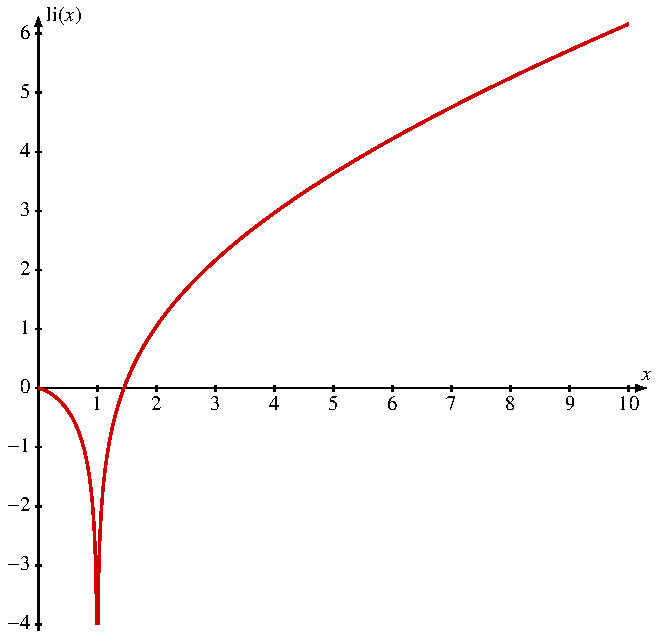
\includegraphics{chapters/070-intalg/images/li.pdf}
\caption{Graph der Integrallogarithmusfunktion
$\operatorname{li}(x)$ für $x>0$.
\label{buch:intalg:fig:li}}
\end{figure}
%
Das bestimmte Integral
\[
\operatorname{li}(x)
=
\int_0^x
\frac{1}{\log t}
\,dt
\]
heisst der \emph{Integrallogarithmus}.
\index{Integrallogarithmus}%
\index{li(x)@$\operatorname{li}(x)$}%
\end{definition}

Eine graphische Darstellung des Graphen von $\operatorname{li}(x)$ ist
in Abbildung~\ref{buch:intalg:fig:li} wiedergegeben.
Da der Integrand an der Stelle $x=1$ eine Singularität hat, muss dieser
Argumentwert mit dem Hauptwert überbrückt werden.
Die Funktion ist daher für $x>1$ durch
\[
\operatorname{li}(x)
=
\lim_{\varepsilon\to 0+}
\biggl(
\int_0^{1-\varepsilon} \frac{dt}{\log t}
+
\int_{1+\varepsilon}^x \frac{dt}{\log t}
\biggr)
\]
definiert.

\begin{beispiel}
Hat die Funktion $1/x\log x \in \mathbb{Q}(x,\log x)$ eine elementare
Stammfunktion?
Mit $\vartheta=\log x$ ist die Stammfunktion des rationalen Teils
\begin{equation}
\frac{1}{x\vartheta}
=
\frac{1/x}{\vartheta}
=
\frac{a(\vartheta)}{b(\vartheta)}
\qquad\Rightarrow\qquad
\begin{cases}
a(\vartheta) &= 1/x\\
b(\vartheta) &= \vartheta
\end{cases}
\label{buch:intalg:risch:eqn:1xlogx}
\end{equation}
nach der Methode von Rothstein-Trager zu bestimmen.
Dazu müssen gemeinsame Teiler von
\[
a(\vartheta) - z\cdot Db(\vartheta)
=
\frac{1}{x} - zD\vartheta
=
\frac{1}{x} - z\frac{1}{x}
\qquad\text{und}\qquad
b(\vartheta)=\vartheta
\]
bestimmt werden.
Da das linke Polynom Grad 0 hat, kann es nur dann nichttriviale
Teiler vom Grad mindestens 1 geben, wenn es verschwindet, wenn also
\[
\frac{1}{x} - z\frac{1}{x}
=
0
\qquad\Rightarrow\qquad
\frac{1-z}{x}
=
0
\qquad\Rightarrow\qquad
c=z=1.
\]
Der gemeinsame Teiler ist $v=\vartheta=\log x$.
Nach der Methode von Rothstein-Trager ist daher
\[
f(x)
=
1\frac{Dv}{v}
=
\frac{1}{x \vartheta}
\qquad\Rightarrow\qquad
\int f
=
\log v
=
\log \vartheta
=
\log\log x,
\]
ein elementare Stammfunktion des Integranden $f$.

Die Wahl $a(\vartheta)=1/x$ in \eqref{buch:intalg:risch:eqn:1xlogx}
wird dadurch festgelegt, dass $b(\vartheta)$ ein normiertes Polynom
sein muss.
Der Faktor $x$ im Nenner von \eqref{buch:intalg:risch:eqn:1xlogx}
kann daher nicht Teil des Polynoms $b(\vartheta)$ sein, sondern muss
in $a(\vartheta)$ integriert werden.
\end{beispiel}

%
% Der polynomielle Teil für logarithmische Erweiterungen
%
\subsubsection{Der polynomielle Teil für logarithmische Erweiterungen}
Wir betrachten wieder die Situation einer logarithmischen Erweiterung
$F(\vartheta)\supset F$ um ein logarithmisches Element $\vartheta =\log u$
mit Konstantenkörper $K$.
Wir versuchen die Stammfunktion des polynomiellen Teils in $F(\vartheta)$
zu bestimmen, den wir als
\begin{equation}
p(\vartheta)
=
p_0 + p_1\vartheta + \dots + p_{l-1}\vartheta^{l-1} + p_l\vartheta^l
\in
F[\vartheta]
\label{buch:intalg:risch:eqn:logpolyintegrand}
\end{equation}
schreiben.
Für ein Polynom in der unabhängigen Variablen $x$ ist die Stammfunktion
trivialerweise elementar, da 
\[
\int p_kx^k \,dx = \frac{p_k}{k+1}z^{k+1} + C
\]
ist.
Dies funktioniert jedoch nur für konstante Koeffizienten.
In der vorliegenden allgemeinen Situation
\eqref{buch:intalg:risch:eqn:logpolyintegrand}
erwarten wir eine wesentlich kompliziertere Lösung.

Falls $p(\vartheta)$ eine elementare Stammfunktion hat, dann muss 
sie nach dem Liouville-Prinzip die Form
\begin{align}
\int p(\vartheta)
&=
v_0(\vartheta) + \sum_{i=1}^n c_i\log v_i(\vartheta)
\notag
\intertext{mit $v_i(\vartheta) \in F(\vartheta)$ und $c_i\in K$ haben.
Wie früher darf man annehmen, dass die $v_i(\vartheta)$ teilerfremde,
quadratfreie Polynome sind.
In der abgeleiteten Form ist}
p(\vartheta)
&=
Dv_0(\vartheta)
+
\sum_{i=1}^n c_i \frac{Dv_i(\vartheta)}{v_i(\vartheta)}.
\notag
\intertext{Auf der linken Seite dieser Gleichung steht ein Polynom,
auf der rechten Seite kommen die Nenner $v_i(\vartheta)$ vor.
Da sie teilerfremd sind, können sich die Brüche nicht wegheben, in den
Termen der Summe darf also $\vartheta$ gar nicht vorkommen.
Es bleibt daher die Form}
p(\vartheta)
&=
Dq(\vartheta) + \sum_{i=1}^n c_i \frac{Dv_i}{v_i}
\notag
\\
&=
D(q_{l+1}\vartheta^{l+1} + q_l\vartheta^l + \dots + q_2\vartheta^2
+ q_1\vartheta) + Dq_0 + \sum_{i=1}^n c_i\frac{Dv_i}{v_i}
\label{buch:intalg:risch:logarithmisch:eqn:pDq}
\end{align}
mit $v_i\in F$, $c_i\in K$ und $q\in F[\vartheta]$.
Die Aufgabe ist, das Polynom $q(\vartheta)$ zu bestimmen.

Der Koeffizient $q_0$ für sich alleine interessiert nicht wirklich,
da für die gesuchte Stammfunktion nur die Kombination
\[
\bar{q}_0
=
q_0 + \sum_{i=1}^n c_i\log v_i
\]
benötigt wird.

Zur Bestimmung der Koeffizienten $q_k$ und $\bar{q}_0$ vergleichen wir
Koeffizienten in 
\eqref{buch:intalg:risch:logarithmisch:eqn:pDq}.
Es ergeben sich die Gleichungen
\begin{align*}
0   &= Dq_{l+1}
	&&\Rightarrow
	& Dq_{l+1} &= 0
\\[-4pt]
p_l &= Dq_l + q_{l+1}(l+1) \frac{Du}{u}
	&&\Rightarrow
	& Dq_l     &= p_l - (l+1)q_{l+1}\frac{Du}{u}
\\[-9pt]
    &\phantom{n}\vdots 
	&&           &
	&\phantom{n}\vdots
\\[-9pt]
p_k &= Dq_k + q_{k+1}(k+1) \frac{Du}{u}
	&&\Rightarrow
	& Dq_k     &= p_k - (k+1)q_{k+1}\frac{Du}{u}
\\[-9pt]
    &\phantom{n}\vdots        
	&&
	&          &\phantom{n}\vdots
\\[-9pt]
p_1 &= Dq_1 + 2q_2 \frac{Du}{u}
	&&\Rightarrow
	& Dq_1     &= p_1 - 2q_2 \frac{Du}{u}
\\[-0pt]
p_0 &= D\bar{q}_0 + q_1 \frac{Du}{u}
	&&\Rightarrow& D\bar{q}_0 &= p_1 - q_1 \frac{Du}{u}
\end{align*}
Die rechten Seiten zeigen, dass alle Koeffizieten von $q(\vartheta)$
als Lösung eines Integrationsproblems im kleineren Körper $F$ gefunden
werden müssen.
Jedes dieser einzelnen Integrationsproblem muss eine elementare
Lösung in $F(\vartheta)$ haben.
Die Lösung des Integrationsproblems für $d_k$ ist aber immer nur bis auf
eine Integrationskonstante $b_k$ bestimmt.

Aus der ersten Gleichung folgt, dass $q_{l+1}$ eine Konstante sein muss,
die mit $b_{l+1}$ bezeichnet wird.
Da $q_{l+1}$ auch in der Gleichung für $q_l$ auftritt, kann
letztere zur Bestimmung von $b_{l+1}$ herangezogen werden.

Die Gleichung für $q_l$ wird mit der Lösung für $q_{l+1}$ zu
\[
Dq_l
=
p_l-(l+1)b_{l+1}\frac{Du}{u}.
\]
Die Lösung muss eine elementare Funktion sein, nach dem Prinzip von Liouville
muss
\[
q_l
=
d_l + c_l\vartheta + b_l
\]
mit $d_l\in F$ und $c_l,b_l\in K$ sein.
Durch Ableiten und Vergleich mit der Gleichung für $Dq_l$ schilessen wir,
dass
\[
p_l - (l+1)b_{l+1}\frac{Du}{u} 
=
Dq_l 
=
Dd_l + c_l\frac{Du}{u}
\qquad\Rightarrow\qquad
\left\{
\;
\renewcommand{\arraycolsep}{2pt}
\begin{array}{rcl}
\displaystyle d_l     &=& \displaystyle \int p_l \\[9pt]
\displaystyle b_{l+1} &=& \displaystyle -\frac{c_{l}}{l+1}.
\end{array}
\right.
\]
sein muss.
Damit ist jetzt auch die Integrationskonstante $b_{l+1}$ bestimmt.

Nehmen wir an, dass die Koeffizienten bis $q_{k+1} = d_{k+1}+b_{k+1}$
bereits bestimmt sind.
Nur die Integrationskonstante $b_{k+1}$ ist noch zu bestimmen.
Die Bestimmungsgleichung
\begin{align*}
Dq_k &= p_k - (k+1) q_{k+1} \frac{Du}{u}
\intertext{wird damit zu}
Dq_k
&=
p_k
-
(k+1) d_{k+1} \frac{Du}{u}
-
(k+1) b_{k+1} \frac{Du}{u}.
\intertext{Der letzte Term kann ist sofort integrierbar, wir können
daher die Terme so sortieren, dass}
p_k
-
(k+1) d_{k+1} \frac{Du}{u}
&=
Dq_k
+
(k+1) b_{k+1} \frac{Du}{u}.
\end{align*}
Die linke Seite muss also eine elementare Stammfunktion haben,
die nach dem Prinzip von Liouville wieder in der Form $d_k + c_k\vartheta$
geschrieben werden kann.
Durch Ableiten und Termvergleich können wir wieder
\[
\left.
\renewcommand{\arraycolsep}{2pt}
\begin{array}{rcl}
d_k
&=&
\displaystyle
\int\biggl(
p_k
-
(k+1) d_{k+1} \frac{Du}{u}
\biggr)
\\[9pt]
b_{k+1}
&=&
\displaystyle
-
\frac{c_k}{k+1}
\end{array}
\;
\right\}
\quad\Rightarrow\quad
q_k = d_k + b_k
\]
schliessen.
Dieser Schritt kann für kleiner werdende $k$ wiederholt werden bis
$q_1=d_1+b_1$ bsetimmt ist, wobei die Integrationskonstante $b_1$ noch
zu finden ist.

%
% polylog.tex
%
% (c) 2026 Prof Dr Andreas müller
%
\begin{figure}
\centering
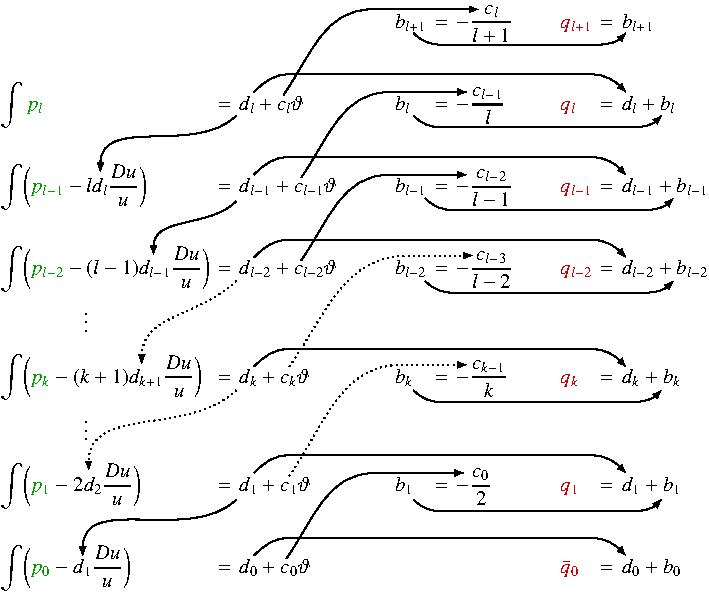
\includegraphics{chapters/070-intalg/images/polylog.pdf}
\caption{Gang der Rechnung für den polynomiellen Teil im Fall einer
logarithmischen Erweiterung.
Aus den bekannten Koeffizienten $p_k\in F$ wird zunächst der Integrand
gebildet, wozu $d_{k-1}$ aus dem vorangegangenen Schritt benötigt wird.
Die Stammfunktion liefert $d_k$ und die Konstante $c_k$, mit der sich
die Integrationskonstaten $b_{k-1}$ im vorangegangenen Schritt
festlegen lässt.
\label{buch:intalg:risch:logarithmisch:fig:polylog}}
\end{figure}
%

Die Bestimmungsgleichung für $\bar{q}_0$ ist
\[
D\bar{q}_0
=
p_0 - q_1\frac{Du}{u}
=
p_0 - d_1\frac{Du}{u} - c_1\frac{Du}{u}
\quad\Rightarrow\quad
D\bar{q}_0
-
c_1\frac{Du}{u}
=
p_0 - d_1\frac{Du}{u}.
\]
Um $\bar{q}_0$ zu bestimmen, muss eine Stammfunktion gefunden werden.
Dazu muss wieder das Integrationsproblem für den Integranden ganz rechts
gelöst werden.
Im Gegensatz zu den früheren Schritten darf die Stammfunktion
\[
\int
\biggl(
p_0 - d_1\frac{Du}{u}
\biggr)
=
d_0
=
v_0 + \sum_{i=1}^m \bar{c}_i \log v_i, \qquad \bar{c}_i\in K
\]
aber auch andere Logarithmen als $\vartheta$ enthalten, solange
sie Logarithmen von Elemente von $F$ sind.
Einer der Logarithmen darf $\vartheta$ sein, sei dies der erste.
Aus der Konstanten $\bar{c}_1$ lässt sich dann auch auch
\(
b_1 = -\bar{c}_1
\)
bestimmen.
Dadurch ist $\bar{q}_0=d_0$ jetzt bis auf eine Konstante unbekannte
Integrationskonstante $b_0$ bestimmt.

Der Gang der Berechnung ist in
Abbildung~\ref{buch:intalg:risch:logarithmisch:fig:polylog} 
schematisch dargestellt.
Im Schritt zur Bestimmung von $q_k$ wird zunächst aus dem bekannten
Koeffizienten $p_k$ und der Stammfunktion $d_{k-1}$ aus dem vorangegangenen
Schritt der Integrand gebildet.
Seine Stammfunktion liefert $d_k$ und die Konsante $c_k$.
Die Integrationskonstante $b_{k-1}$ im vorangegangenen Schritt ist
durch $c_k$ bestimmt.
Schliesslich kann $q_k = d_k+b_k$ gefunden werden.
Nur die letzte Integrationskonstante $b_0$ kann nicht bestimmt werden.

\begin{beispiel}
Man finde die Stammfunktion von $f(x) = \log x$.
Der Integrand ist das Polynom
\[
f(x)=\vartheta
=
1\cdot\vartheta + 0
=
p_1\vartheta + p_0
\qquad\Rightarrow\qquad
\begin{cases}
p_1 &= 1\\
p_0 &= 0.
\end{cases}
\]
in der Erweiterung
$F(\vartheta)=\mathbb{Q}(x,\vartheta)$ von $F=\mathbb{Q}(x)$ um das
logarithmische Element $\vartheta=\log x$.
Es muss also ein Polynom
\[
q(\vartheta)
=
q_2\vartheta^2 + q_1\vartheta + \bar{q}_0
\]
vom Grad 2 gefunden werden.
\begin{itemize}
\item Fall $k=2$:
$q_2$ muss eine Konstante $b_2$ sein, deren Wert im
nächsten Schritt bestimmt wird.
\item Fall $k=1$:
Zur Bestimmung von $q_1$ muss zunächst die Stammfunktion
von $p_1$ bestimmt werden, sie ist
\[
\int p_1
=
\int 1
=
x + 0\cdot\vartheta
\quad
\Rightarrow
\quad
\left\{
\quad
\renewcommand{\arraycolsep}{2pt}
\begin{array}{rcl}
b_2 &=& \displaystyle -\frac{c_1}{2} \\
d_1 &=& x
\end{array}
\quad
\right\}
\quad
\Rightarrow
\quad
q_1 = x + b_1
\]
Da darin $\vartheta$ nicht vorkommt, folgt $c_1=0$ und daher $b_2=0$.
Die Integrationskonstante $b_1$ wird im nächsten Schritt bestimmt.
\item Fall $k=0$:
Es muss die Stammfunktion von $p_0-d_1\,Du/u$ aus
\[
q_0
=
\int\biggl(p_0-d_1\frac{Du}u\biggr)
=
\int\biggl(0-x\frac{1}{x}\biggr)
=
-
\int 1
=
-x
+
b_0
=
d_0+b_0
\]
bestimmt werden.
Auch hier kann man schliessen, dass $b_1=0$ ist.
\end{itemize}
Aus den drei Fällen lässt sich jetzt die Stammfunktion
\[
\int p(\vartheta)
=
q(\vartheta)
=
q_0 + q_1\vartheta + q_2\vartheta^2
=
-x+b_0 + z\vartheta
=
x\log x - x + b_0
\]
ablesen.
Tatsächlich ist die Ableitung davon
\[
\frac{d}{dx}\bigl( x\log x - x + b_0\bigr)
=
\log x + x \frac 1x - 1
=
\log x.
\]
Wie erwartet kann die Integrationskonstante $b_0$ nicht bestimmt werden.
\end{beispiel}

\begin{beispiel}
Hat der Integrand $\log\log x$ eine elementare Stammfunktion?
Für diese Aufgabe muss der Körper der rationalen Funktionen zweimal
logarithmisch erweitert werden, zunächst um $\vartheta_1=\log x$ und
dann im zweiten Schritt um $\vartheta_2 = \vartheta =\log u = \log\log x$.
Gesucht ist jetzt das Integral des Polynoms
$p(\vartheta) = 1\cdot\vartheta + 0$
mit $p_1=1$ und $p_0=0$.
\begin{itemize}
\item Fall $k=2$:
$q_2$ muss eine Konstante $b_2$ sein, deren Wert im
nächsten Schritt bestimmt wird.
\item Fall $k=1$:
Die Stammfunktion $p_1$ ist
\[
\int p_1
=
\int 1
=
x + 0\cdot \vartheta
\quad
\Rightarrow
\quad
\left\{
\quad
\renewcommand{\arraycolsep}{2pt}
\begin{array}{rcl}
b_2 &=& \displaystyle -\frac{c_1}{2} \\
d_1 &=& x
\end{array}
\quad
\right\}
\quad
\Rightarrow
\quad
q_1 = x + b_1
\]
Wie früher folgt $c_1=0$ und $b_2=0$.
Die Integrationskonstante $b_1$ wird im nächsten Schritt bestimmt.
\item Fall $k=0$: Es ist die Stammfunktion von $p_0-d_1 \, Du/u$ zu bestimmen:
\[
q_0
=
\int\biggl(p_0-d_1\frac{Du}u\biggr)
=
\int\biggl(0-x \frac{D\log x}{\log x}\biggr)
=
-\int x \frac{1/x}{\log x}
=
-
\int 
\frac{1}{\log x}.
\]
Dieses Integral ist nach
Beispiel~\ref{buch:intalg:risch:bsp:1/logx}
nicht elementar und daher kann auch das Integral von $\log\log x$ nicht
elementar sein.
\qedhere
\end{itemize}
\end{beispiel}

%
% Anwendung: Der Satz von Hardy-Littlewood
%
\subsubsection{Anwendung: Der Satz von Littlewood-Hardy}
Warum ist
\begin{align}
\int \frac{\log x}{x}\,dx
&=
\frac12\log(x)^2+C
\label{buch:intalg:risch:littlewood-hardy:bsp1}
\intertext{elementar, während}
\int \frac{\log x}{x+1}\,dx
&=
\log(x)\log(x+1) + \operatorname{Li}_2(-x)+C
\label{buch:intalg:risch:littlewood-hardy:bsp2}
\end{align}
keine elementare Stammfunktion hat?
Mit der für den polynomiellen Teil einer logarithmischen Erweiterung
entwickelten Methode lässt sich diese Frage für allgemeinere
Integrale der Form
\[
\int f(x)\log x \,dx
\qquad\text{mit } f(x)\in K(x)
\]
entscheiden.
Offensichtlich geht es hier um die logarithmische Erweiterung
$\vartheta=\log x $ von $K(x)$.
Der Integrand $f(x)\log(x)$ ist der Fall eines polynomiellen Teils
für das Polynom $p(\vartheta) = f(x)\vartheta$ mit $p_1=f(x)$.
Wenn eine elementare Stammfunktion existiert, dann hat sie die
Form eines Polynoms
$q(\vartheta) = q_2\vartheta^2 + q_1\vartheta + q_0\in F[\vartheta]$
vom Grad $\le 2$.
Wir berechnen die Koeffizienten $q_k$:
\begin{itemize}
\item
Fall $k=2$: 
$q_2$ muss eine Konstante $b_2$ sein, deren Wert im nächsten Schritt
bestimmt wird.

\item
Fall $k=1$:
Für $q_1$ muss die Stammfunktion von $p_1$ bestimmt werden.
Nach dem Liouville-Prinzip muss sie die Form
\begin{align}
\int f(x)\,dx
&=
v_0(x) + \sum_{i=1}^n c_i\log v_k(x)
\notag
\intertext{haben.
Damit die Methode für den polynomiellen Teil aufgeht, darf in der Summe
nur ein einziger Logarithmus $\log x $ vorkommen, also}
&=
v_0(x) + c_1\log x
\label{buch:intalg:risch:littlewood-hardy:eqn:condition}
\end{align}
mit $v_1(x)=\log x=\vartheta$.
Es folgt $b_2=-\frac12c_1$ und $d_1=v_0(x)$ und $q_1 = v_0(x) + b_1$.
Die Integrationskonstante $b_1$ wird im nächsten Schritt bestimmt.

Die in
\eqref{buch:intalg:risch:littlewood-hardy:eqn:condition}
bedeutet nach Ableitung, dass
\[
f(x) = v_0'(x) + \frac{c_1}{x}
=
g'(x) + \frac{C}{x}
\]
mit einer rationalen Funktion $g(x)$.

\item
Fall $k=0$: Es muss die Stammfunktion von $p_0-d_1\,Du/u$ ermittelt
werden, die die Form
\[
\int p_0 - d_1\frac{Du}{u}
=
-
\int v_0(x) \frac{1}{x}
=
d_0 + c_0\vartheta
\]
haben muss.
Da $v_0(x)/x$ eine rationale Funktion ist, existiert diese Stammfunktion
in der Form
\begin{equation}
\int v_0(x)\frac1x\,dx
=
u_0(x) + \sum_{i=1}^m \tilde{c}_k \log \tilde{u}_k(x).
\label{buch:intalg:risch:littlewood-hardy:eqn:q0}
\end{equation}
Es folgt $d_0=u_0(x)$.
Falls eine der Funktion $\tilde{u}_k(x)=x$ ist, kann der zugehörige
Koeffizient $\tilde{c}_k$ als $c_0$ verwendet und bestimmt damit $b_1$.

Da das Integral~\eqref{buch:intalg:risch:littlewood-hardy:eqn:q0} immer
ausführbar ist, auferlegt der Fall $k=0$ keine zusätzlichen Hindernisse
für die Existenz einer elementaren Stammfunktion.
\end{itemize}

Die Existenz einer elementaren Stammfunktion lässt sich also für Integranden
der Form $f(x)\log x$ immer entscheiden.
Wir fassen die Erkenntnisse der Methode im folgenden Satz zusammen.

\begin{satz}[Littlewood-Hardy]
\index{Satz!von Littlewood-Hardy}%
\index{Littlewood, John Endsor}%
\index{Hardy, Harold Godrey}%
Für eine rationale Funktion $f(x)\in K(x)$ hat der Integrand $f(x)\log x$
genau dann eine elementare Stammfunktion, wenn es eine rationale Funktion
$g(x)\in\mathbb K(x)$ gibt derart, dass
\[
f(x) = g'(x) + \frac{C}{x}.
\]
\end{satz}

\begin{beispiel}
Das Integral \eqref{buch:intalg:risch:littlewood-hardy:bsp1} ist
der Fall $f(x)=1/x$, es muss also untersucht werden, ob es eine rationale
Funktion $g(x)$ und eine Konstante $C$ gibt mit
\[
f(x) = \frac{1}{x} = g'(x) + \frac{C}{x}.
\]
$g(x)=0$ und $C=1$ ist eine offensichtliche Lösung, also ist die Stammfunktion
von $\log(x)/x$ elementar.
Tatsächlich ist
\[
\int\frac{\log x}{x}\,dx
=
\frac{\log(x)^2}{2}
+ C.
\qedhere
\]
\end{beispiel}

\begin{beispiel}
Das Integral \eqref{buch:intalg:risch:littlewood-hardy:bsp2} ist
der Fall $f(x)=1/(x+1)$, es muss also untersucht werden, ob es eine rationale
Funktion $g(x)$ und eine Konstante $C$ gibt mit
\[
f(x) = \frac{1}{x+1} = g'(x) + \frac{C}{x}.
\]
Aufgelöst nach $g'(x)$ ist dies
\[
g'(x) = \frac{1}{x+1} - \frac{C}{x}
\quad\Rightarrow\quad
g(x)
=
\log(x+1) -C\log x + D.
\]
Da $g(x)$ keine rationale Funktion ist, kann das Integral von $f(x)$ 
nicht elementar sein.
\end{beispiel}

%
% Risch-Algorithmus für exponentielle Erweiterungen
%
\subsection{Risch-Algorithmus für exponentielle Erweiterungen
\label{buch:intalg:risch:exponentiell}}
Abschnitt~\ref{buch:intalg:risch:logarithmisch} hat für den Fall einer
logarithmischen Erweiterung die Lücken in der allgemeinen Beschreibung
des Algorithmus in Abschnitt~\ref{buch:intalg:risch:uebersicht} gefüllt.
In diesem Abschnitt soll das Gleiche für eine exponentielle Erweiterung
getan werden.
Sei im Folgenden also $\vartheta=e^u$ ein Logarithmus eines Elements
$u\in F$.
Sie ist charakterisiert durch $D\vartheta = \vartheta\cdot Du$.

%
% Die Methode von Hermite
%
\subsubsection{Die Methode von Hermite}
In der Methode von Hermite wird benötigt, dass $b(\vartheta)$ und
$Db(\vartheta)$ teilerfremd sind.
Da $b(\vartheta)$ quadratfrei ist, sind $b(\vartheta)$ und $b'(\vartheta)$
teilerfremd.

\begin{lemma}
\label{buch:intalg:risch:exp:lemma:bDb}
Sei $b(\vartheta)\in F[\vartheta]$ ein quadratfreies Polynom.
Dann sind $b(\vartheta)$ und $Db(\vartheta)$ genau dann teilerfremd,
wenn $\vartheta$ kein Teiler von $b(\vartheta)$ ist.
\end{lemma}

\begin{proof}
Wie im Beweis von Lemma~\ref{buch:intalg:risch:log:lemma:bDb} verwenden
wir eine Faktorisierung
\[
b(\vartheta) = \prod_{i=1}^m (\vartheta-\beta_i)
\]
mit der Ableitung
\[
Db(\vartheta)
=
\sum_{k=1}^m D(\vartheta-\beta_i)\prod_{i\ne k} (\vartheta-\beta_i).
\]
Sei wieder $\vartheta-\beta_j$ ein gemeinsamer Teiler von $b(\vartheta)$
und $Db(\vartheta)$.
Dann folgt wie im Beweis von Lemma~\ref{buch:intalg:risch:log:lemma:bDb},
dass $\vartheta-\beta_j$ ein Teiler von $D(\vartheta-\beta_j)$ sein muss.
Nach dem Satz~\ref{buch:intalg:liouville:polynome:satz:logarithmisch} ist
$(\vartheta-\beta_j)\mid (D\vartheta-D\beta_j)$ genau dann, wenn der Teiler ein
Monom ist, wenn also $\beta_j=0$ und damit $\vartheta$ ein Teiler von
$b(\vartheta)$ ist.
\end{proof}

Das Lemma zeigt also, dass die Teilerfremdheit von $b(\vartheta)$ und
$Db(\vartheta)$ genau dann folgt, wenn $b(\vartheta)$ nicht durch
$\vartheta$ teilbar ist.
Schliesst man Faktoren $\vartheta$ im Nenner aus, kann die Methode von
Hermite durchgeführt werden und die Stammfunktion kann mit der Methode
von Rothstein-Trager gefunden werden.

%
% Erweiterte Polynome
%
\subsubsection{Erweiterte Polynome}
Die Diskussion der Methode von Hermite für exponentielle Erweiterungen
hat gezeigt, dass der Faktor $\vartheta$ im Nenner separat behandelt
werden muss.
Ein Faktor $\vartheta$ ist aber sehr leicht am Verschwinden des
Terms vom Grad 0 in einem Polynom erkennbar, so dass die Faktoren $\vartheta$
in der Faktorisierung
\[
q(\vartheta)
=
\vartheta^l \cdot b_1(\vartheta) b_2(\vartheta)^2 \cdots b_m(\vartheta)^m
\]
des Nenners als separate Faktoren behandelt werden können.
Die Faktoren $b_k(\vartheta)$ sind quadratfrei und nicht durch $\vartheta$
teilbar.

Die Partialbruchzerlegung von $r(\vartheta)/q(\vartheta)$ hat dann die
Form
\begin{align}
\frac{r(\vartheta)}{b(\vartheta)}
&=
\sum_{i=1}^l \frac{a_i}{\vartheta^i}
+
\sum_{i=1}^m
\sum_{k=1}^{\deg b_i(\vartheta)}
\frac{a_{ik}(\vartheta)}{b_i(\vartheta)^k}
\label{buch:intalg:risch:exp:eqn:partbruch}
\end{align}
mit $a_i\in F$ und $a_{ik}\in F[\vartheta]$.
Die zweite Summe in \eqref{buch:intalg:risch:exp:eqn:partbruch}
enthält nur Terme, die den Faktor $\vartheta$ im 
Nenner nicht enthalten und daher mit der Methode von Hermite
reduziert werden können.

Die erste Summe in \eqref{buch:intalg:risch:exp:eqn:partbruch}
kann nicht mit der Methode von Hermite reduziert werden.
Im Fall rationaler Funktionen wären die Terme $1/z^i$ mindestens
für $i\ne 1$ auch sehr einfach mit der Stammfunktion
\[
\int \frac{1}{z^i}
=
\int z^{-i}
=
\frac{1}{-i+1}
z^{-i+1}
=
\frac{1}{(1-i)z^{i-1}}
\]
zu finden, die ein Erweiterung der Regel für Potenzen ist.
Man könnte die Terme $a_i/\vartheta^i$ daher zum polynomiellen
Teil schlagen.
Wir definieren dazu verallgemeinerte Polynome wie folgt.

\begin{definition}[verallgemeinertes Polynom]
Ein \emph{verallgemeinertes Polynom} in $\vartheta$ mit Koeffizienten
\index{verallgemeinertes Polynom}%
\index{Polynom!verallgemeinert}%
in $F$ ist eine Summe der Form
\[
p(\vartheta)
=
\sum_{i=-k}^l p_i\vartheta^i.
\]
Verallgemeinerte Polynome werden auch \emph{Laurent-Polynome} genannt.
\index{Laurent-Polynom}%
Das Paar $(l,k)=\deg p(\vartheta)$ heisst der \emph{Grad} des verallgemeinerten
Polynoms.
Wir nennen $l$ auch den \emph{negativen Grad} und $k$ den
\emph{positiven Grad}.
\index{negativer Grad}%
\index{Grad!negativ}%
\index{positiver Grad}%
\index{Grad!positiv}%
\end{definition}

Die später zu entwickelnde Methode für den polynomiellen Teil muss also
nicht nur mit Polynomen, sondern mit verallgemeinerten Polynomen umgehen
können.

\begin{lemma}
\label{buch:intalg:risch:lemma:verallgabl}
Die Ableitung eines verallgemeinerten Polynoms $p(\vartheta)$ ist
wieder ein verallgemeinertes Polynom mit den gleichen Graden.
\end{lemma}

\begin{proof}
Wir berechnen zunächst die Ableitung
\begin{align}
Dp(\vartheta)
&=
\sum_{i=-k}^l Dp_i\vartheta^i
+
\sum_{i=-k}^l p_i i \vartheta^{i-1} \vartheta Du
\notag
\\
&=
\sum_{i=-k}^l Dp_i\vartheta^i
+
\sum_{i=-k}^l p_i i \vartheta^i Du
\notag
\\
&=
\sum_{i=-k}^l (Dp_i + ip_i Du ) \vartheta^i.
\label{buch:intalg:risch:lemma:eqn:verallgabl}
\end{align}
Wegen $Dp_i+ip_iDu\in F$ ist 
\eqref{buch:intalg:risch:lemma:eqn:verallgabl}
ein verallgemeinertes Polynom.

Für den höchsten Koeffizienten $Dp_l +lp_lDu$ folgt wie im Beweis
von Satz~\ref{buch:intalg:liouville:polynome:satz:exponentiell},
dass dieser nicht verschwinden kann und der positive Grad von
$p(\vartheta)$ und $Dp(\vartheta)$ gleich sind.

Wäre $\bar{p}_{-k}=Dp_{-k} -k p_k Du=0$, dann wäre auch
\[
D(p_{-k}\vartheta^{-k})
=
\bar{p}_{-k}\vartheta^n
=
0,
\]
insbesondere müsste $p_{-k}\vartheta^{-k}=c$ eine Konstante sein.
Dann wäre aber auch
\[
c\vartheta^k - p_{-k}=0,
\]
und somit wäre $\vartheta$ ein algebraisches Element, im Widerspruch
dazu, dass $\vartheta$ transzendent ist.
Der Widerspruch zeigt, dass auch der negative Grad gleich ist.
\end{proof}

%
% Der Beweis von Lemma 8.27
%
\subsubsection{Der Beweis von Lemma~\ref{buch:intalg:risch:lemma:v0exp}}

\begin{proof}[Beweis von Lemma~\ref{buch:intalg:risch:lemma:v0exp}]
Wegen $v_0(\vartheta)=F(\vartheta)$ dürfen wir annehmen, dass
\[
v_0(\vartheta) = \frac{p(\vartheta)}{q(\vartheta)}
\]
mit teilerfremden Polynomen $p(\vartheta),q(\vartheta)\in F[\vartheta]$
und $q(\vartheta)$ normiert.
Die Ableitung ist
\begin{equation}
Dv_0(\vartheta)
=
\frac{Dp(\vartheta)}{q(\vartheta)}
-
\frac{p(\vartheta)\cdot Dq(\vartheta)}{q(\vartheta)^2}.
\label{buch:intalg:risch:lemma827:Dv0}
\end{equation}
Nach Satz~\ref{buch:intalg:liouville:polynome:satz:exponentiell} sind
$Dp(\vartheta)$ und $Dq(\vartheta)$ wieder Polynome vom gleichen Grad.
Da die linke Seite von \eqref{buch:intalg:risch:rt:eqn:liouvillediff}
und die Terme $Dv_k(\vartheta)/v_k(\vartheta)$
einen quadratfreien Nenner haben, muss auch der Nenner von
\eqref{buch:intalg:risch:lemma827:Dv0} quadratfrei sein.
Im Gegensatz zur Argumentation im Beweis von
Lemma~\ref{buch:intalg:risch:lemma:v0log} kann das bei einer
exponentiellen Erweiterung auch dadurch erreicht werden, dass
$q(\vartheta)\mid Dq(\vartheta)$, dann folgt nach
Satz~\ref{buch:intalg:liouville:polynome:satz:exponentiell} aber,
dass $q(\vartheta)=\vartheta^n$ ist.
Wir schliessen daher, dass
\[
v_0(\vartheta)
=
\sum_{i=-s}^t p_i\vartheta^i
\]
ein verallgemeinertes Polynom ist und müssen nur noch zeigen, dass $s=t=0$ ist.

Die Ableitung eines verallgemeinerten Polynoms ist nach
Lemma~\label{buch:intalg:risch:lemma:verallgabl}
wieder ein verallgemeinertes Polynome mit dem gleichen Grad, in
Satz~\ref{buch:intalg:liouville:polynome:satz:exponentiell}
wurde dafür die Notation
\[
Dv_0(\vartheta)
=
\sum_{i=-s}^t \bar{p}_i\vartheta^i
\]
verwendet.

Da weder in der linken Seite von \eqref{buch:intalg:risch:lemma827:Dv0}
noch in den Termen $Dv_k(\vartheta)/v_k(\vartheta)$ der Nenner $\vartheta$
vorkommt, darf er auch in $Dv_0(\vartheta)$ nicht vorkommen.
Es folgt $s=0$.

Bringt man die rechte Seite von \eqref{buch:intalg:risch:lemma827:Dv0}
auf einen gemeinsamen Nenner, muss der Grad des Zählers kleiner sein als
der Grad des Nenners, weil dies auf der linken Seite der Fall ist.
Alle Terme $Dv_k(\vartheta)/v_k(\vartheta)$ haben gleichen Zähler- und
Nennergrad.
Die genannte Bedingung kann also nur erfüllt werden, wenn $t=0$ ist.
\end{proof}

%
% Rothstein-Trager für exponentielle Erweiterungen
%
\subsubsection{Rothstein-Trager für exponentielle Erweiterungen}
Der Satz~\ref{buch:intalg:risch:satz:rothstein-trager-logarithmisch}
von Rothstein-Trager für logarithmische Erweiterungen hat im Beweis
wesentlich zwei früher bewiesene Eigenschaften verwendet.
Einerseits war bereits bekannt, dass der Term $v_0$ in der
Stammfunktion verschwindet.
Ausserdem wurde verwendet, dass Ableiten den Grad eines normierten
Polynoms immer verkleinert.
Beide Voraussetzungen sind bei einer exponentiellen Erweiterung
nicht mehr gegeben.
Trotzdem werden wir unten einen analogen Satz für exponentielle
Erweiterungen beweisen.

Die Ableitung eines normierten Polynoms 
\begin{align*}
p(\vartheta)
&=
p_0 + p_1\vartheta + p_2\vartheta^2 + \ldots + p_{n-1}\vartheta^{n-1} + \vartheta^n
\intertext{ist}
Dp(\vartheta)
&=
Dp_0 + (Dp_1+ p_1Du)\vartheta + (Dp_2+2p_2Du)\vartheta^2 + \ldots
\\
&\qquad
+ (Dp_{n-1}+(n-1)p_{n-1}Du)\vartheta^{n-1} + nDu \vartheta^n.
\end{align*}
Der Term höchsten Grades ist $(\deg p(\vartheta))Du$.
Genau dieser Term verhindert, dass der Grad des Zählers abnimmt, was im
Beweis von Satz~\ref{buch:intalg:risch:satz:rothstein-trager-logarithmisch}
zum Beweis von $\bar{a}(\vartheta)=a(\vartheta)$ verwendet worden war.

\begin{definition}[Führender Term eines Polynoms]
Sei $p(\vartheta)\in F[\vartheta]$ ein Polynom vom Grad $n$ mit Koeffizienten
$p_i$, $i=1,\dots,n$,
dann heisst
\[
l(p(\vartheta))
=
p_n\vartheta^n
=
p_{\deg p(\vartheta)} \vartheta^{\deg p(\vartheta)}
\]
der \emph{führende Term}.
\index{fuhrender Term@führender Term}
\end{definition}

Für zwei beliebige Polynome $p(\vartheta),q(\vartheta)\in F[\vartheta]$ gilt
$l(p(\vartheta)q(\vartheta)) = l(p(\vartheta)) l(q(\vartheta))$.
Für die Polynome $v_k(\vartheta)$ folgen die Formeln
\begin{align*}
l(b(\vartheta))
&=
\prod_{i=1}^m l(v_i(\vartheta)),
&
l(u_k(\vartheta))
&=
\prod_{\scriptstyle i=1\atop\scriptstyle i\ne k} l(v_i(\vartheta))
&&\text{und}&
l(v_k(\vartheta)) l(u_k(\vartheta)) &= l(b(\vartheta)).
\end{align*}
Da die Polynome $v_k(\vartheta)$ und $b(\vartheta)$ normiert sind,
ist $l(v_k(\vartheta)) = \vartheta^{\deg v_k(\vartheta)}$ und
$l(b(\vartheta))=\vartheta^{\deg b(\vartheta)}$.
Für eine exponentielle Erweiterung und ein normiertes Polynome ist zudem
\begin{equation}
l(Dp(\vartheta))) = \deg p(\vartheta) l(p(\vartheta)) Du.
\end{equation}

Wir wissen bereits, dass die Stammfunktion die Form
\eqref{buch:intalg:risch:satz:eqn:standardform}
haben muss, müssen aber den Term $v_0$ noch bestimmen.
Die Brüche $Dv_k(\vartheta)/v_k(\vartheta)$ enthalten als
Term höchsten Grades
$l(Dv_k(\vartheta))=(\deg v_k(\vartheta))Du \vartheta^{\deg v_k(\vartheta)}$
im Zähler.
Wir können versuchen, diese Terme zum Verschwinden zu bringen, indem wir 
sie mithilfe des Terms $v_0$ wieder subtrahieren.
Dazu muss $v_0$ den Teil
\[
g = -\biggl(\sum_{i=1}^m c_i\deg v_i(\vartheta)\biggr) u
\]
enthalten.

\begin{satz}[Rothstein-Trager]
\label{buch:intalg:risch:satz:rothstein-trager-exponentiell}
Seien
\[
f = \frac{a(\vartheta)}{b(\vartheta)},
\qquad
a(\vartheta),b(\vartheta)\in F[\vartheta],\quad
\deg a(\vartheta)<\deg b(\vartheta)
\]
und $b(\vartheta)$ quadratfrei, normiert und $\vartheta$ teilt $b(\vartheta)$
nicht.
Dann gilt:
\begin{enumerate}
\item $f$ hat eine elementare Stammfunktion genau dann, wenn die $z$,
für die 
\begin{equation}
a(\vartheta)-z\cdot Db(\vartheta)
\qquad\text{und}\qquad
b(\vartheta)
\label{buch:intalg:risch:exp:eqn:rtggt}
\end{equation}
einen nichttrivialen gemeinsamen Teiler haben, Konstanten $c_i \in K$ sind.
\item Die Stammfunktion ist in diesem Fall
\[
\int f
=
g
+
\sum_{i=1}^n c_i \log v_i(\vartheta),
\]
wobei $v_i(\vartheta)$ der zu $c_i$ gehörige grösste gemeinsame Teiler
der Polynome~\eqref{buch:intalg:risch:exp:eqn:rtggt} und
\begin{equation}
g = -\biggl(\sum_{i=1}^n c_i\deg v_i(\vartheta) \biggr) u
\quad\text{mit Ableitung}\quad
Dg = -\biggl(\sum_{i=1}^n c_i\deg v_i(\vartheta) \biggr) Du
\label{buch:intalg:risch:exp:eqn:g}
\end{equation}
ist.
\end{enumerate}
\end{satz}

\begin{proof}
Wie im Beweis von
Satz~\ref{buch:intalg:risch:satz:rothstein-trager-logarithmisch}
setzen wir
\begin{equation}
\bar{a}(\vartheta)
=
g b(\vartheta)
+
\sum_{i=1}^m c_i b(\vartheta) \frac{Dv_i(\vartheta)}{v_i(\vartheta)}
=
-g b(\vartheta)
+
\sum_{i=1}^m c_i Dv_i(\vartheta) u_i(\vartheta)
\label{buch:intalg:risch:exp:rt:eqn:abar}
\end{equation}
und zeigen wieder, dass $\bar{a}(\vartheta)=a(\vartheta)$.

Für jedes $k$ ist
\begin{align*}
\bar{a}(\vartheta)
-
c_k Db(\vartheta)
=
gb(\vartheta)
+
\sum_{\scriptstyle i=1\atop\scriptstyle i\ne k}^m
(c_i-c_k) Dv_i(\vartheta) u_i(\vartheta).
\end{align*}
Auf der rechten Seite verschwindet der Summand mit $i=k$.
$v_k(\vartheta)$ teilt $b(\vartheta)$ und jeden Faktor $u_i(\vartheta)$
für $i\ne k$.
Somit teilt 
\begin{align*}
v_k(\vartheta) &\mid (\bar{a}(\vartheta)-c_k Db(\vartheta)) \\
v_k(\vartheta) &\mid (     a (\vartheta)-c_k Db(\vartheta))
\intertext{und daher auch}
v_k(\vartheta) &\mid (\bar{a}(\vartheta)-a(\vartheta)).
\intertext{Weil die $v_k(\vartheta)$ teilerfremd sind folgt auch}
b(\vartheta) &\mid (\bar{a}(\vartheta)-a(\vartheta)).
\end{align*}

Der Term höchsten Grades in $c_i Dv_i(\vartheta) u_i(\vartheta)$ ist
\begin{align*}
l(c_i Dv_i(\vartheta) u_i(\vartheta))
&=
c_i l(Dv_i(\vartheta)) l(u_i(\vartheta))
\\
&=
c_i \deg v_i(\vartheta) l(v_i(\vartheta)) Du l(u_i(\vartheta))
\\
&=
c_i \deg v_i(\vartheta) l(b(\vartheta)) Du.
\end{align*}
Alle Summanden in \eqref{buch:intalg:risch:exp:rt:eqn:abar} haben
den gleichen Grad.
Die Terme in der Summe haben daher zusammen den führenden Term
\[
l\biggl(
\sum_{i=1}^m c_i Dv_i(\vartheta) u_i(\vartheta)
\biggr)
=
\sum_{i=1}^m c_i\deg v_i(\vartheta) l(b(\vartheta)) Du
=
-l(gb(\vartheta))
=
-g\vartheta^{\deg b(\vartheta)}.
\]
Der führend Term fällt daher in $\bar{a}(\vartheta)$ weg und es folgt
$\deg \bar{a}(\vartheta) < \deg b(\vartheta)$.

Wir haben gezeigt, dass $b(\vartheta)$ Teiler des Polynoms
$\bar{a}(\vartheta)-a(\vartheta)$ kleineren Grades ist, somit
muss $\bar{a}(\vartheta)-a(\vartheta)=0$ sein.
Damit ist beweisen, dass $\bar{a}(\vartheta)=a(\vartheta)$ ist.
\end{proof}

\begin{beispiel}
\label{buch:intalg:risch:exp:bsp:1/ex+1}
Man finde eine Stammfunktion der Funktion
\[
f
=
\frac{1}{e^x+1}
=
\frac{1}{\vartheta + 1},
\]
wobei $\vartheta=e^x$ eine exponentielle Erweiterung ist.
\medskip

\noindent
Der Nenner $b(\vartheta) = \vartheta+1$ ist nicht durch $\vartheta$ teilbar,
somit ist die Methode von Rothstein-Trager anwendbar.
Wegen $a(\vartheta)=1$ muss $z$ so bestimmt werden, dass
\[
a(\vartheta) - z\cdot Db(\vartheta)
=
1- z \cdot D\vartheta
=
1- z\cdot \vartheta Du
=
1-z\cdot \vartheta 
\qquad\text{und}\qquad
b(\vartheta) = \vartheta+1
\]
einen nichttrivialen gemeinsamen Teiler haben.
Beide Polynome sind vom Grad 1, ein gemeinsamer Teiler ist also nur
möglich, wenn die Polynome Vielfache voneinander sind.
Dies ist der Fall, wenn $z=c_1=-1$ ist.
Der grösste gemeinsame Teiler ist dann $v_i=\vartheta+1$.

Die Funktion $g$ in \eqref{buch:intalg:risch:exp:eqn:g}
ist
\[
g
=
-\biggl(\sum_{i=1}^n c_i\deg v_i \biggr) u
=
- c_1 \deg v_1 u
=
x.
\]
Es folgt, dass
\begin{equation}
\int\frac{1}{e^x+1}
=
g+
c_1\log v_i
+
c_0
=
x
-\log (e^x+1)
+
c_0.
\label{buch:intalg:risch:exp:eqn:intf}
\end{equation}
Tatsächlich ist die Ableitung der rechten Seite
\[
D
\bigl(
x
-\log (e^x+1)
+
c_0
\bigr)
=
1
-D\log(e^x+1)
=
1
-\frac{D(e^x+1)}{e^x+1}
=
\frac{e^x+1-e^x}{e^x+1}
=
\frac{1}{e^x+1},
\]
was die Korrektheit der Stammfunktion
\eqref{buch:intalg:risch:exp:eqn:intf}
bestätigt.
\end{beispiel}

\begin{beispiel}
\label{buch:intalg:risch:exp:bsp:x/ex+1}
Man finde eine Stammfunktion von 
\begin{equation}
f = \frac{x}{e^x+1} = \frac{x}{\vartheta+1},
\label{buch:intalg:risch:exp:eqn:x/ex+1}
\end{equation}
wobei $\vartheta$ die exponentielle Erweiterung mit $\vartheta=e^x$.
\medskip

\noindent
Wie in Beispiel~\ref{buch:intalg:risch:exp:bsp:1/ex+1} ist
$b(\vartheta)=\vartheta+1$ quadratfrei, normiert und nicht durch $\vartheta$
teilbar, die Methode von Rothstein-Trager ist daher anwendbar.
Gesucht sind diejenigen $z$, für die
\[
a(\vartheta) - z\cdot Db(\vartheta)
=
x- z \cdot D\vartheta
=
x- z\cdot \vartheta Du
=
x-z\cdot \vartheta 
\qquad\text{und}\qquad
b(\vartheta) = \vartheta+1
\]
einen nichttrivialen gemeinsamen Teiler haben.
Wieder ist dies nur möglich, wenn das linke Polynom ein Vielfaches
des rechten Polynoms ist.
Dies ist genau für $z=c_1=-x$ der Fall, dann ist
\[
a(\vartheta) - z\cdot Db(\vartheta)
=
x+x \vartheta 
=
x(\vartheta+1)
\]
ist.
Da $c_1=x$ nicht konstant ist, kann es keine elementare Stammfunktion
geben.
\end{beispiel}

Da der Integrand~\eqref{buch:intalg:risch:exp:eqn:x/ex+1} keine
elementare Stammfunktion hat, ist die Definition einer neuen
speziellen Funktion angebracht, mit der die Stammfunktion ausgedrückt
werden kann.

\begin{definition}[Dilogarithmus]
Der \emph{Dilogarithmus} ist die Funktion
\[
\operatorname{Li}_2(z)
=
\sum_{k=1}^\infty \frac{z^k}{k^2}
\]
für $|z|<1$.
\index{Dilogarithmus}%
\end{definition}

Die Ableitung des Dilogarithmus ist
\begin{equation}
\frac{d}{dz}
\operatorname{Li}_2(z)
=
\sum_{k=1}^\infty \frac{z^{k-1}}{k}
=
\frac{1}{z}
\sum_{k=1}^\infty \frac{z^k}{k}
=
-
\frac{ \log(1-z) }{z},
\label{buch:intalg:exp:dilog:integraldef}
\end{equation}
wobei der letzte Schritt aus der Potenzreihenentwicklung
\[
\log(1+z) = -\sum_{k=1}^\infty (-1)^k\frac{z^k}{k}
\qquad\Rightarrow\qquad
-\log(1-z) = \sum_{k=1}^\infty \frac{z^k}{k}
\]
des Logarithmus folgt, die durch gliedweise Integration der geometrischen
Reihe
\begin{align*}
\frac{1}{1+z}
&=
\sum_{k=0}^\infty (-1)^kz^k
\\
\Rightarrow\qquad
\int\frac{dz}{1+z}
=
\log(1+z)
&=
\sum_{k=0}^\infty (-1)^{k+1}z^{k+1}
=
\sum_{k=1}^\infty (-1)^k z^k
\end{align*}
gefunden werden kann.
%
% fig-li2.tex -- Graph der Funktion Li_2(x)
%
% (c) 2026 Prof Dr Andreas Müller
%
\begin{figure}
\centering
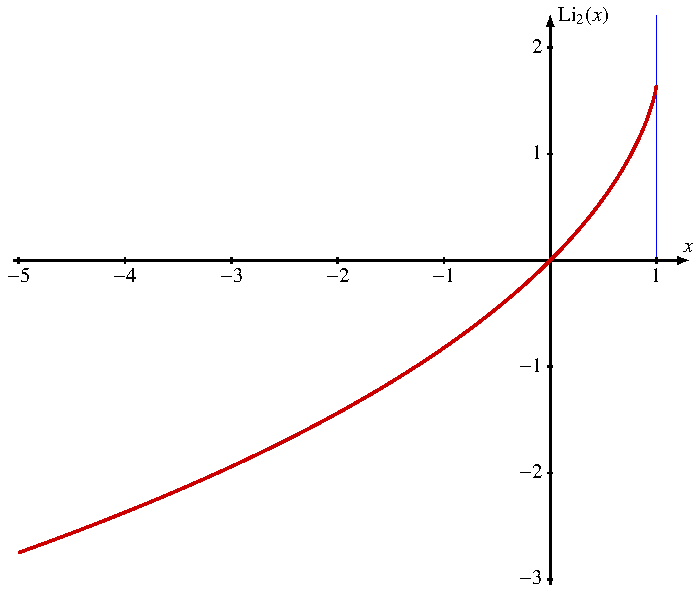
\includegraphics{chapters/070-intalg/images/li2.pdf}
\caption{Graph der Dilogarithmusfunktion
$\operatorname{Li}_2(x)$ für $x<1$.
\label{buch:intalg:fig:li2}}
\end{figure}
%
Aus der Ableitung~\eqref{buch:intalg:exp:dilog:integraldef}
folgt die Integraldefinition
\[
\operatorname{Li}_2(x)
=
-\int_0^x
\frac{\log(1-t)}{t}\,dt
\]
des Dilogarithmus für reelle Argumente $x\in(-\infty,0)$, die als
Basis für die graphische Darstellung des Graphen von
$\operatorname{Li}_2(x)$ 
in Abbildung~\ref{buch:intalg:fig:li2} diente.

Damit kann jetzt die Stammfunktion von $f(x)=x/(e^x+1)$ bestimmt werden.
Mathematica findet die Funktion
\index{Mathematica}%
\begin{align*}
F(x)
&=
-x\log(1+e^{-x})
+
\operatorname{Li}_2(-e^{-x}).
\intertext{Um davon die Ableitung zu berechnen, ist es nützlich, die
Ableitung von $\operatorname{Li}_2(-e^{-x})$ haben.
Sie ist}
\frac{d}{dx}
\operatorname{Li}_2(-e^{-x})
&=
\log(1+e^{-x}).
\intertext{Die Ableitung von $F(x)$ wird damit}
\frac{d}{dx}F(x)
&=
-\log(1+e^{-x})
-x\frac{1}{1+e^{-x}}\frac{d}{dx}(e^{-x})
+
\log(1+e^{-x})
\\
&=
-
\log(1+e^{-x})
+
x\frac{1}{1+e^{-x}}e^{-x}
+
\log(1+e^{-x})
\\
&=
x\frac{e^{-x}}{1+e^{-x}}.
\intertext{Erweitern mit $e^x$ ergibt}
&=
\frac{x}{e^x+1}.
\end{align*}
Damit ist gezeigt, dass $F(x)$ tatsächlich die Stammfunktion von $f(x)$
ist.

Das Computeralgebrasystem Maxima findet eine auf den ersten Blick gänzlich
andere Stammfunktion, nämlich
\begin{align}
G(x)
&=
\frac{x^2}2 - x \log(e^x+1) - \operatorname{Li}_2(-e^{x}).
\notag
\intertext{In diesem Fall brauchen wird die Ableitung}
\frac{d}{dx}\operatorname{Li}_2(-e^x)
&=
-\log(e^x+1).
\intertext{Die Ableitung von $G(x)$ wird damit}
\frac{d}{dx}G(x)
&=
x-\log(e^x+1) - \frac{xe^x}{e^x+1} 
+
\log(e^x+1)
\notag
\\
&=
\frac{x(e^x+1)-xe^x}{e^x+1} 
\notag
\\
&=
\frac{x}{e^x+1}.
\end{align}
Auch diese Form der Stammfunktion ist also korrekt.

Die beiden Stammfunktionen $F(x)$ und $G(x)$ können sich um höchstens
eine Konstante unterscheiden, die Differenz ist 
\begin{align}
C
=
F(x)-G(x)
&=
-x\log(1+e^{-x})+\operatorname{Li}_2(-e^{-x})
-\frac{x^2}2+x\log(e^x+1)+\operatorname{Li}_2(-e^x)
\notag
\intertext{Die Konstante kann durch Evaluieren für $x=0$ gefunden werden,
sie stellt sich als $C=0$ heraus.
Die beiden Logarithmus-Terme können als Logarithmus eines Bruchs
geschrieben werden:}
0
&=
-x\log\frac{1+e^{-x}}{e^x+1}+\operatorname{Li}_2(-e^{-x})
-\frac{x^2}2+\operatorname{Li}_2(-e^x)
\notag
\\
&=
-x\log e^{-x}
-
\frac{x^2}2
+
\operatorname{Li}_2(-e^{-x})
+
\operatorname{Li}_2(-e^x)
\notag
\\
0
&=
\frac{x^2}2
+
\operatorname{Li}_2(-e^{-x})
+
\operatorname{Li}_2(-e^x),
\label{buch:intalg:risch:li2identity}
\end{align}
eine nichttriviale Identität für den Dilogarithmus.

Die Ableitung von
$
\operatorname{Li}_2(-e^{-x})
+
\operatorname{Li}_2(-e^x)
$
ist
\begin{align*}
\frac{d}{dx}\Bigl(
\operatorname{Li}_2(-e^{-x})
+
\operatorname{Li}_2(-e^x)
\Bigr)
&=
\log(1+e^{-x})-\log(e^x+1)
\\
&=
\log\frac{1+e^{-x}}{e^x+1}
=
\log e^{-x}
=
-x
\end{align*}
mit der Stammfunktion $-\frac{x^2}{2}$, was 
\eqref{buch:intalg:risch:li2identity}
bestätigt.

%
% Der polynomielle Teil und die Risch-Differentialgleichung
%
\subsubsection{Der polynomielle Teil und die Risch-Differentialgleichung}
Der polynomielle Teil des Integranden $f\in F(\vartheta)$ ist eine 
erweitertes Polynom der Form
\[
p(\vartheta)
=
\sum_{i=-k}^l
p_i\vartheta^i,
\]
dessen Stammfunktion jetzt analog zum logarithmischen Fall durch
Koeffizientenvergleich ermittelt werden soll.

Die Ableitung eines Monoms ist
\[
D(a\vartheta^n) 
=
(Da)\vartheta^n + an\vartheta^{n-1}D\vartheta
=
(Da)\vartheta^n + an\vartheta^{n-1}\vartheta Du
=
(Da + naDu)\vartheta^n,
\]
also wieder ein Monom mit dem gleichen Exponenten.
Die Ableitung reduziert im Gegensatz zum logarithmischen Fall den
Grad nicht.
Man darf daher erwarten, dass die Stammfunktion wieder ein erweitertes
Polynom
\[
q(\vartheta)
=
\sum_{i=-k}^l q_i\vartheta^i
\]
ist.

Um die Koeffizienten des Polynoms zu finden, leiten wir $q(\vartheta)$
ab und führen Koeffizientenvergleich in
\[
p(\vartheta)
=
\sum_{i=-k}^l p_i\vartheta^i
=
Dq\vartheta
=
\sum_{i=-k}^l
(Dq_i + iq_i Du)\vartheta^i
\]
durch.
Es ergeben sich die Differentialgleichungen
\begin{equation}
Dq_i + iDu\cdot q_i = p_i
\label{buch:intalg:risch:exponentiell:eqn:rischdgl}
\end{equation}
für $i =-k,\dots, l$.
Gesucht sind Lösungen $q_i\in F$.
Falls es keine solche Lösung gibt, hat $p(\vartheta)$ keine elementare
Stammfunktion.

Auf den ersten Blick scheint es, dass die Differentialgleichung
\eqref{buch:intalg:risch:exponentiell:eqn:rischdgl}
das Integrationsproblem in eine Differentialgleichungsproblem
umwandelt.
Die Bestimmung einer Stammfunktion ist ein Spezialfall der Lösung
einer Differentialgleichung, man könnte also meinen, dass das
ursprüngliche Problem durch ein schwierigeres Problem ersetzt worden
ist.
Zudem sagen doch die bekannten Sätze aus der Theorie der gewöhnlichen
Differentialgleichungen, dass die Lösung mindestens lokal existiert
und eindeutig ist.
Es geht aber nicht darum, eine beliebige Lösungsfunktion zu finden,
sondern diese Funktion muss in $F$ sein.
Der Satz von Picard-Lindelöf als Beispiel eines Existenz- und
Eindeutigkeitssatzes für gewöhnliche Differentialgleichungen
kann dazu nichts aussagen.
Daher wurden auch gänzlich andere Methoden zur Lösung dieser
Differentialgleichung entwickelt.

\begin{definition}[Risch-Differentialgleichung]
Sei $F$ ein differentieller Funktionenkörper und $f,g\in F$.
Das Problem, eine Lösung $y\in F$ der Differentialgleichung
\[
Dy + f\, y = g
\]
zu finden, heisst die \emph{Risch-Differentialgleichung}.
\end{definition}

\begin{beispiel}
Hat die Wahrscheinlichkeitsdichte $e^{-x^2/2}$ eine elementare
Stammfunktion?
Der Integrand ist in der Erweiterung $F(\vartheta)=K(x,\vartheta)$
von $F=K(x)$ um die Exponentialfunktion $\vartheta = e^{-x^2/2}$
von $u=-x^2/2$.
Gesucht ist die Stammfunktion des polynomiellen Teils
$p(\vartheta)=p_1\vartheta^1$.
Sie muss die Form $q_1\vartheta$ haben.
Die Risch-Differentialgleichung ist
\[
Dq_1 + Du\, q_1 = p_1
\quad\Rightarrow\quad
Dq_1 - x q_1 = 1.
\]
Die Lösung muss eine rationale Funktion $q_1\in K(x)$ sein.
Wir schreiben die rationale Funktion als gekürzten Bruch
\begin{equation}
q_1(x) = \frac{a(x)}{b(x)}
\label{buch:intalg:risch:exponentiell:bsp:eqn:qex2}
\end{equation}
von Polynomen $a,b\in K[x]$, $b(x)$ soll ausserdem normiert sein.
Einsetzen in die Differentialgleichung liefert
\begin{align}
\frac{a'(x)b(x)-a(x)b(x)}{b(x)^2} - x\frac{a(x)}{b(x)} &= 1.
\notag
\intertext{Multiplizieren mit dem Nenner $b(x)^2$ führt auf die
Polynomgleichung}
a'(x)b(x) - a(x)b'(x) -x a(x)b(x) &= b(x)^2.
\label{buch:intalg:risch:exponentiell:eqn:qex2poly}
\end{align}
Das Polynom $b(x)$ ist ein Teiler des ersten und des letzten Terms auf
der linken Seite.
Ausserdem teilt es die rechte Seite.
Daher muss es auch den mittleren Term $a(x)b'(x)$ teilen.
Es kann aber keine gemeinsamen Faktoren mit $a(x)$ haben, da angenommen
wurde, dass der Bruch \eqref{buch:intalg:risch:exponentiell:bsp:eqn:qex2}
gekürzt ist.
Es folgt, dass $b(x)$ die Ableitung $b'(x)$ teilt, was nur möglich ist,
wenn $b'(x)=0$ ist.
Das Polynom $b(x)$ ist also nur ein Konstante $b_0$.
Da $b(x)$ ausserdem normiert ist, muss $b_0=1$ sein.

Die Polynomgleichung \eqref{buch:intalg:risch:exponentiell:eqn:qex2poly}
wird jetzt zu
\begin{equation}
a'(x) - x a(x) = 1.
\label{buch:intalg:risch:exponentiell:bsp:eqn:qex2:adgl}
\end{equation}
Schreibt man die Koeffizienten des Polynoms als $a_k$, wird die
Gleichung
\eqref{buch:intalg:risch:exponentiell:bsp:eqn:qex2:adgl}
zu
\begin{align*}
\sum_{k=0}^n ka_kx^{k-1} -x \sum_{k=0}^n a_kx^k &= 1
\\
\sum_{k=1}^n ka_kx^{k-1} - \sum_{k=0}^n a_kx^{k+1} &= 1
\\
\sum_{i=0}^{n-1} (i+1)a_{i+1}x^i - \sum_{i=1}^{n+1} a_{i-1} x^i &= 1
\\
a_1 + \sum_{i=1}^{n-1} \bigl((i+1)a_{i+1}-a_{i-1}\bigr) x^i
+ a_{n-1}x^n + a_{n}x^{n+1} &= 1
\end{align*}
Durch Koeffizientenvergleich liest man die Gleichungen
\begin{align}
a_1 &= 1 \notag \\
(i+1)a_{i+1} -a_{i-1} &= 0 &&\Rightarrow& a_{i-1} &= (i+1)a_{i+1}&&1\le i\le n-1
\label{buch:intalg:risch:exponentiell:bsp:exp2:rekursion}
\\
a_{n-1} &= 0 \notag \\
a_n &= 0 \notag
\end{align}
für die Koeffizienten $a_k$ ab.

Anwendung der Gleichung
\eqref{buch:intalg:risch:exponentiell:bsp:exp2:rekursion} auf
die letzten beiden Bedingungen erlaubt zu schliessen, dass alle
Koeffizienten verschwinden müssen, auch $a_0$.
Dies steht im Widerspruch zur ersten Gleichung $a_1=1$.
Der Widerspruch zeigt, dass die Lösung der Differentialgleichung
keine rationale Funktion sein kann und dass somit auch $e^{-x^2/2}$ keine
elementare Stammfunktion haben kann.
\end{beispiel}

%
% Anwendung: Integration der trigonometrischen Funktionen
%
\subsubsection{Anwendung: Integration der trigonometrischen Funktionen}
Die trigonemetrischen Funktion $\cos x$ und $\sin x$ liegen in der
exponentiellen Erweiterung $\mathbb{Q}(i,x,\vartheta)$ mit
$\vartheta=e^{ix}$.
Wie in Abschnitt \ref{buch:intalg:section:elementar} gezeigt wurde,
ist
\begin{align*}
\cos x
&=
\frac{\vartheta+1/\vartheta}{2}
=
\frac{\vartheta^2+ 1}{\vartheta}
=
\frac12\vartheta + \frac{1/2}{\vartheta}
\\
\sin x
&=
\frac{1}{2i}\vartheta
-
\frac{1/2i}{\vartheta}.
\end{align*}
Man beachte, dass beide Ausdrücke verallgemeinerte Polynome sind.
Zur Bestimmung der Stammfunktion von $\cos x$ sind also die
Risch-Differentialgleichungen
für das Polynom mit den Koeffiziente $p_1=\frac12$ und $p_{-1}=\frac12$
zu lösen:
\begin{align*}
Dq_{\pm 1} \pm i q_{\pm 1} = \frac12
\end{align*}
hat die konstante Lösung $q_{\pm 1} = \pm\frac{1}{2i}$.
Die Stammfunktion ist daher
\[
\int\cos x
=
q_1\vartheta + q_{-1}\frac{1}{\vartheta}
=
\frac{1}{2i}\biggl(\vartheta-\frac1{\vartheta}\biggr)
=
\sin x.
\]
Analog findet man auch die Stammfunktion von $\sin x$.
Der Algorithmus reproduziert also die bekannten Integrationsformeln für
die grundlegenden trigonometrischen Funktionen.

Für die Tangensfunktion gilt
\[
\tan x
=
-i
\frac{\vartheta-1/\vartheta}{\vartheta+1/\vartheta}
=
-i
\frac{\vartheta^2-1}{\vartheta^2+1}
=
-i
+\frac{2i}{\vartheta^2+1}.
\]
Auf den letzten Bruch kann die Methode von Rothstein-Trager angewendet
werden.
Es müssen gemeinsame Teiler von
\[
2i - ic\cdot 2\vartheta^2
=
2i(1-c\vartheta^2)
\qquad\text{und}\qquad
\vartheta^2+1
\]
gefunden werden.
Ein nichttrivialer gemeinsamer Teiler existiert für $c=-1$ und der grösste
gemeinsame Teiler ist $\vartheta^2+1$.
Somit ist
\[
\int \frac{2i}{\vartheta^2+1} = -\log(\vartheta^2+1)
\]
Es folgt, dass
\[
\int \tan x
=
-ix
-
\log(e^{2ix} + 1)
=
\log(e^{-ix})
-
\log(e^{2ix}+1)
=
\log\frac{e^{-ix}}{e^{2ix}+1}
=
\log\frac{1}{e^{ix}+e^{-ix}},
\]
was bis auf eine Konstante mit $\log(\sec(x))$ übereinstimmt.


%
% Risch-Algorithmus für algebraische Erweiterungen
%
\subsection{Risch-Algorithmus für algebraische Erweiterungen
\label{buch:intalg:risch:algebraisch}}
Die Methoden, die für logarithmische und exponentielle Erweiterungen
konstruiert wurden, lassen sich nicht direkt auf algebraische
Erweiterungen übertragen.
Dies deutet sich bereits im Beweis des Liouville-Prinzips für algebraische
Erweiterungen an.
Dort wurde zum Beispiel das Konzept der konjugierten Elemente und andere
rein algebraische Eigenschaften verwendet.

Die bisher in Abschnitt~\ref{buch:intalg:section:risch} verwendeten
Methoden basieren wesentlich darauf, dass sich Polynome in $\vartheta$
auf eindeutige Art faktorisieren lassen.
Der euklidische Algorithmus ist für alle Argumente zentral.
Für eine algebraische Erweiterung gilt dies nicht mehr.

Abschnitt~\ref{buch:intalg:section:wurzel} hat aber gezeigt, dass
eine ähnliche Vorgehensweise denkbar ist, um ein Stammfunktion
einer Funktion in $K(x,y)$ zu finden, wobei $y$ ein über $K(x)$
algebraisches Element ist.
Im einfachsten Fall erfüllt $y$ die Gleichung
\[
y^n - h(x) = 0
\]
mit $h(x) \in K(x)$, $y$ ist also eine $n$-te Wurzel einer rationalen
Funktion.

Ein Beispiel sind die in Kapitel~\ref{chapter:elliptisch} diskutierten
\emph{elliptischen Integrale}
\index{elliptisches Integral}%
\[
f(x) = \int_0^x R(t,\!\sqrt{P(t)})\,dt
\]
in denen $p(t)$ ein Polynom vom Grad 3 oder 4 ist.
Der Fall eines Polynoms vom Grad 2 wurde bereits im
Abschnitt~\ref{buch:intalg:section:wurzel} behandelt.

Zunächst muss man eine gute ``Standarddarstellung'' für eine Funktion
$f\in K(x,y)$ finden.
Bei transzendenten Erweiterungen war die Darstellung als gekürzter Bruch
von Polynomen in $\vartheta$ eindeutig, dies gilt für algebraische
Funktionen nicht mehr.
Man wird also zusätzliche Forderungen an Zähler und Nenner aufstellen
müssen, um eine eindeutige Darstellung zu bekommen.

Für die elliptischen Integrale kann man zum Beispiel zeigen, dass sich
jedes elliptische Integral auf die grundlegenden elliptischen Integrale
\begin{align*}
\text{1.~Art:}&&
F(x;k)
&=
\int_0^{\sin x} \frac{dt}{\!\sqrt{(1-t^2)(1-k^2t^2}}
\\
\text{2.~Art:}&&
E(x;k)
&=
\int_0^{\sin x} \frac{\!\sqrt{1-k^2t^2}}{\!\sqrt{1-t^2}}\,dt
\\[5pt]
\text{3.~Art:}&&
\Pi(n,x;k)
&=
\int_0^{\sin x}\frac{dt}{(1-nt^2)\!\sqrt{(1-t^2)}\!\sqrt{1-k^2t^2}}
\end{align*}
zurückführen lässt.

Des Weiteren muss ein Reduktionsverfahren ähnlich dem Verfahren von
Hermite gefunden werden, welches Integrale von rationalen Funktionen
in $K(x,y)$ auf solche von Brüchen mit besonders einfachen Nennern
reduziert.
Die Schwierigkeit dabei ist, dass der euklidische Algorithmus, der
in der Methode von Hermite von zentraler Bedeutung war, nicht mehr
zur Verfügung steht.

Schliesslich müssen die Koeffizienten der logarithmischen Terme
in der Liouville-Form eines Integrals gefunden werden.
Dazu ist ein Prinzip ähnlich der Methode von Rothstein-Trager
nötig.
Die dazu notwendigen Methoden basieren auf der Idee eines Divisors
aus der algebraischen Geometrie.
Damit würden wir aber den Bereich der Analysis auf so grundlegende
Weise verlassen, dass wir uns mit einem Verweis auf die Literatur
begnügen.
\cite{buch:algorithms} enthält eine kurze Skizze der Problem, die 
zu lösen sind und verweist auf weitere relevante Spezialliteratur.









